\documentclass[10pt,twocolumn,letterpaper]{article}

\usepackage{3dv}
\usepackage{times}
\usepackage{epsfig}
\usepackage{graphicx}
\usepackage{amsmath}
\usepackage{amssymb}

% Include other packages here, before hyperref.

% If you comment hyperref and then uncomment it, you should delete
% egpaper.aux before re-running latex.  (Or just hit 'q' on the first latex
% run, let it finish, and you should be clear).
\usepackage[pagebackref=true,breaklinks=true,letterpaper=true,colorlinks,bookmarks=false]{hyperref}


%\threedvfinalcopy % *** Uncomment this line for the final submission

\def\threedvPaperID{****} % *** Enter the 3DV Paper ID here
\def\httilde{\mbox{\tt\raisebox{-.5ex}{\symbol{126}}}}

% Pages are numbered in submission mode, and unnumbered in camera-ready
\ifthreedvfinal\pagestyle{empty}\fi
\begin{document}

%-------------------------------------------------------------------------
%%%%%%%%% TITLE
\title{Plant Leaf Meshes from RGB-D Sensors}

\author{ 
Daniel Morris \and Saif Imran \and Vincent Zickefoose \and Jin Chen \and David Kramer\\
%Need to fix the following:
Department of Electrical and Computer Engineering\\
Department of Energy Plant Research Laboratory\\
Michigan State University, East Lansing, MI 48824, USA
}

\maketitle

%-------------------------------------------------------------------------
\begin{abstract}

\end{abstract}
%-------------------------------------------------------------------------

\section{Introduction}
\label{sec:intro}

%

%In order to identify energy-related gene functions, plant researchers seek to understand genetic underpinnings of plant growth [REF] and seeking to develop new varieties [REF], 

In order to meet the increasing needs for food and materials, researchers aim to produce sustainable plants with high yield and high resource-use efficiency by testing approaches ranging from molecular biology to field management~\cite{walter2015plant1}. In this process high-throughput plant phenotyping is the major bottleneck~\cite{cobb2013next}. New automated methods to non-invasively measure plant phenotypes including growth, plant structure, leaf layout and orientations, photosynthesis and productivity, are highly expected~\cite{leister1999large,muller2015leaf,walter2015plant1}. 


\begin{figure}
\begin{center}
\begin{tabular}{ c c }
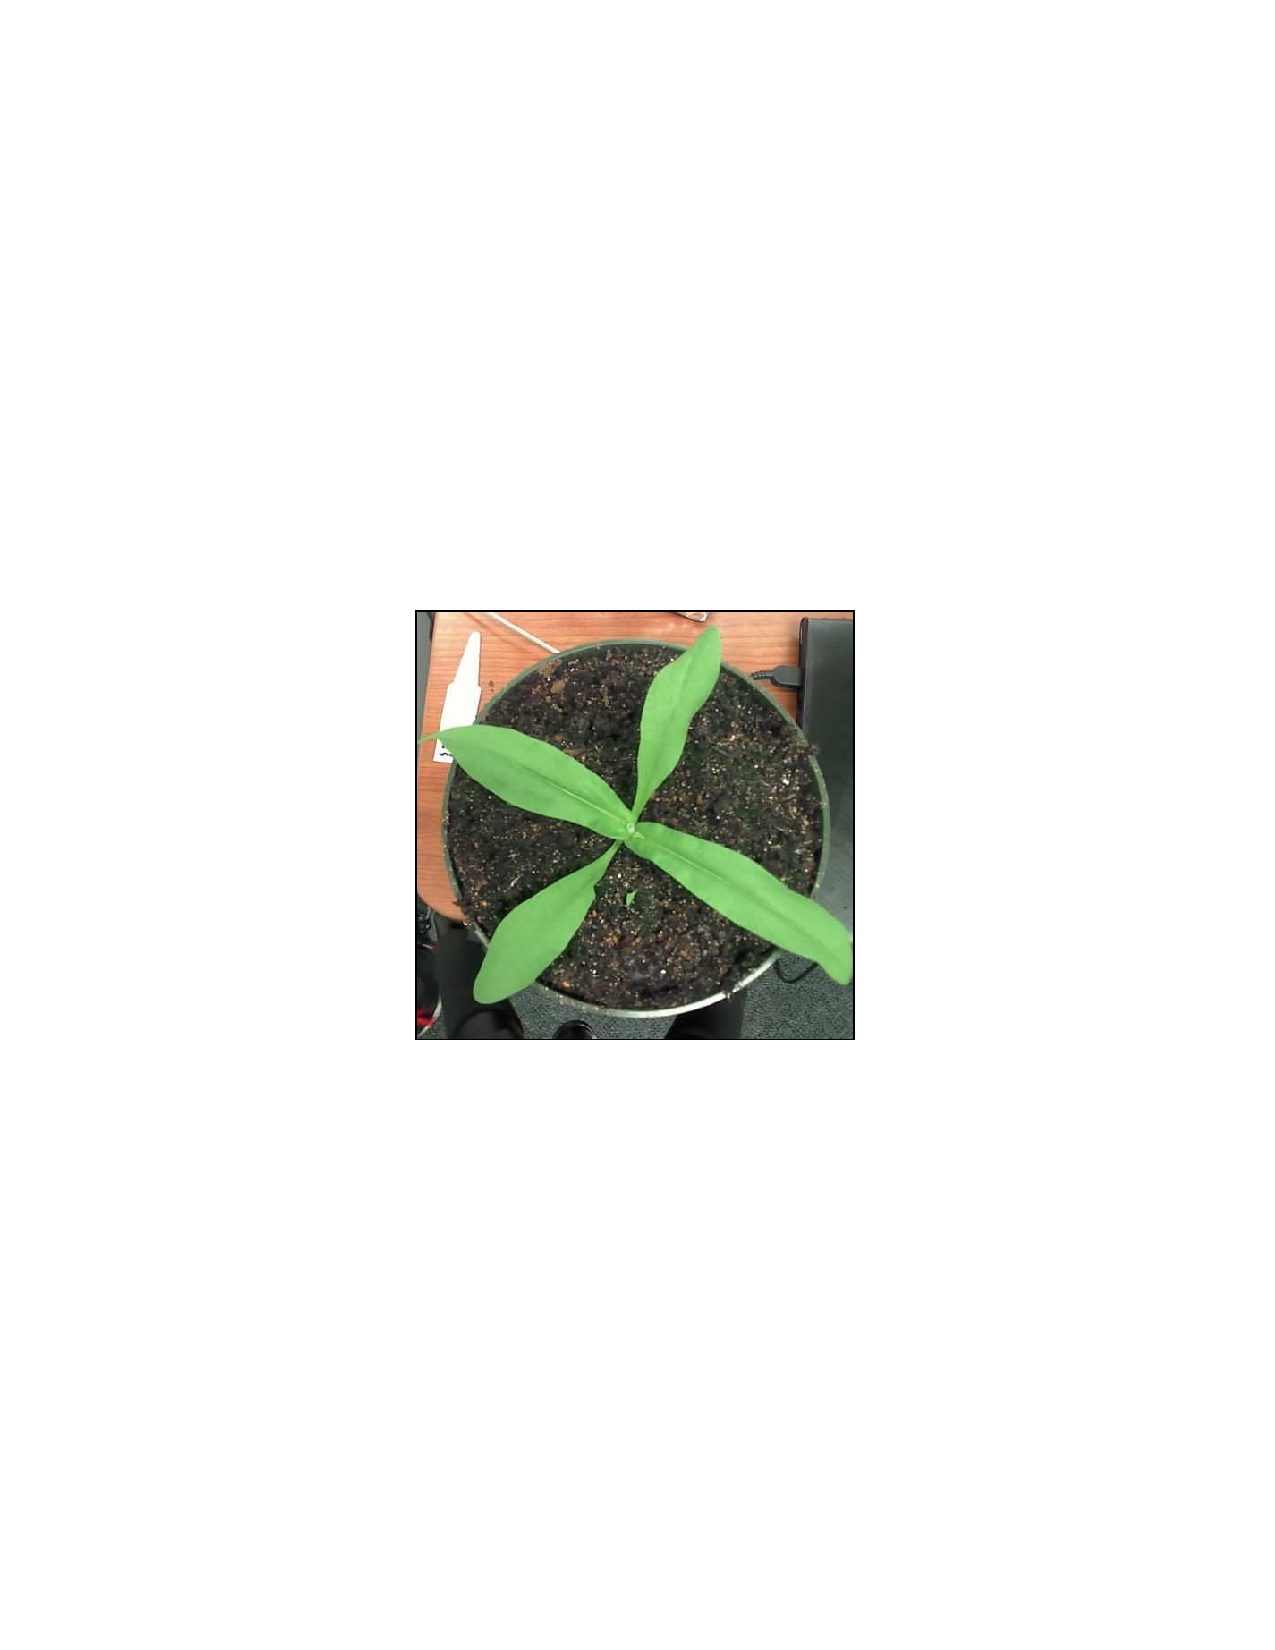
\includegraphics[trim=200 280 200 280,clip,width=0.4\linewidth]{Figures/plant1-rgb} &
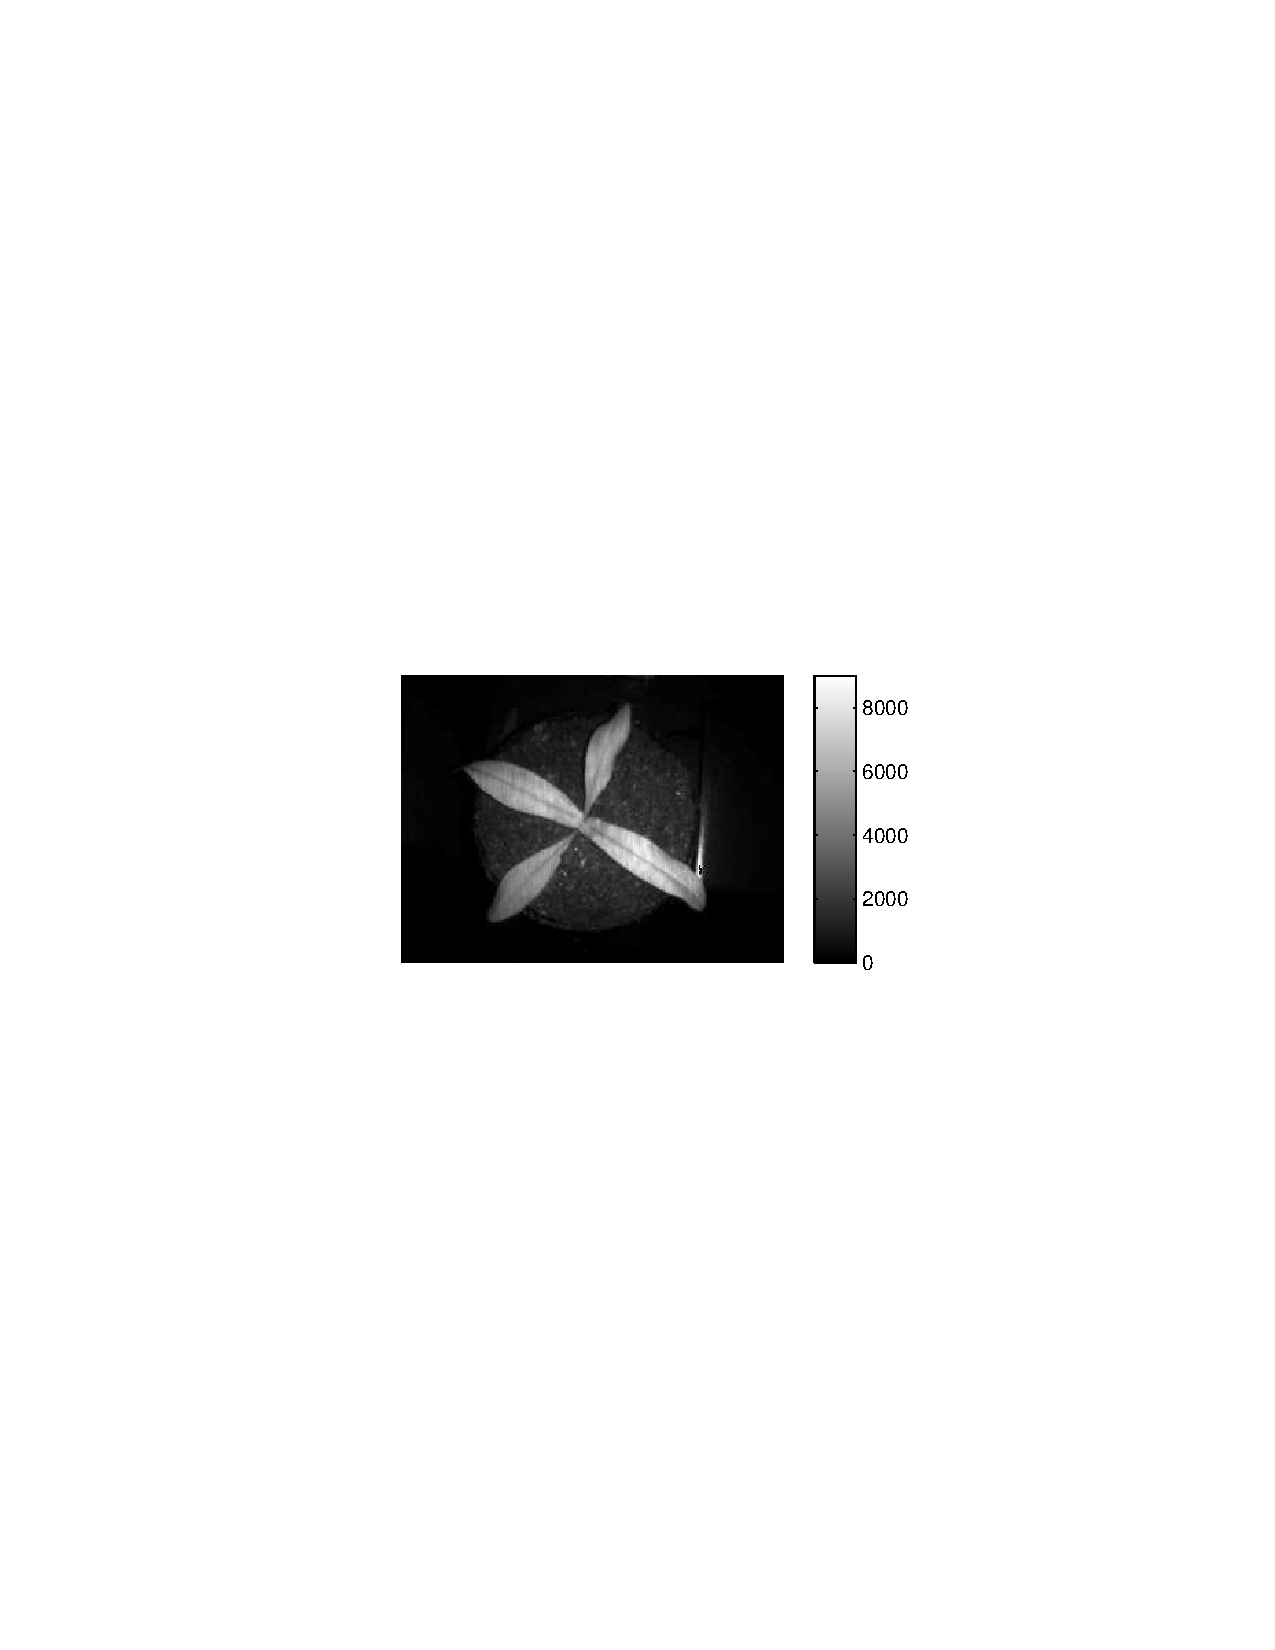
\includegraphics[trim=220 270 160 280,clip,width=0.4\linewidth]{Figures/plant1-ir} \\
($a$) & ($b$) \\
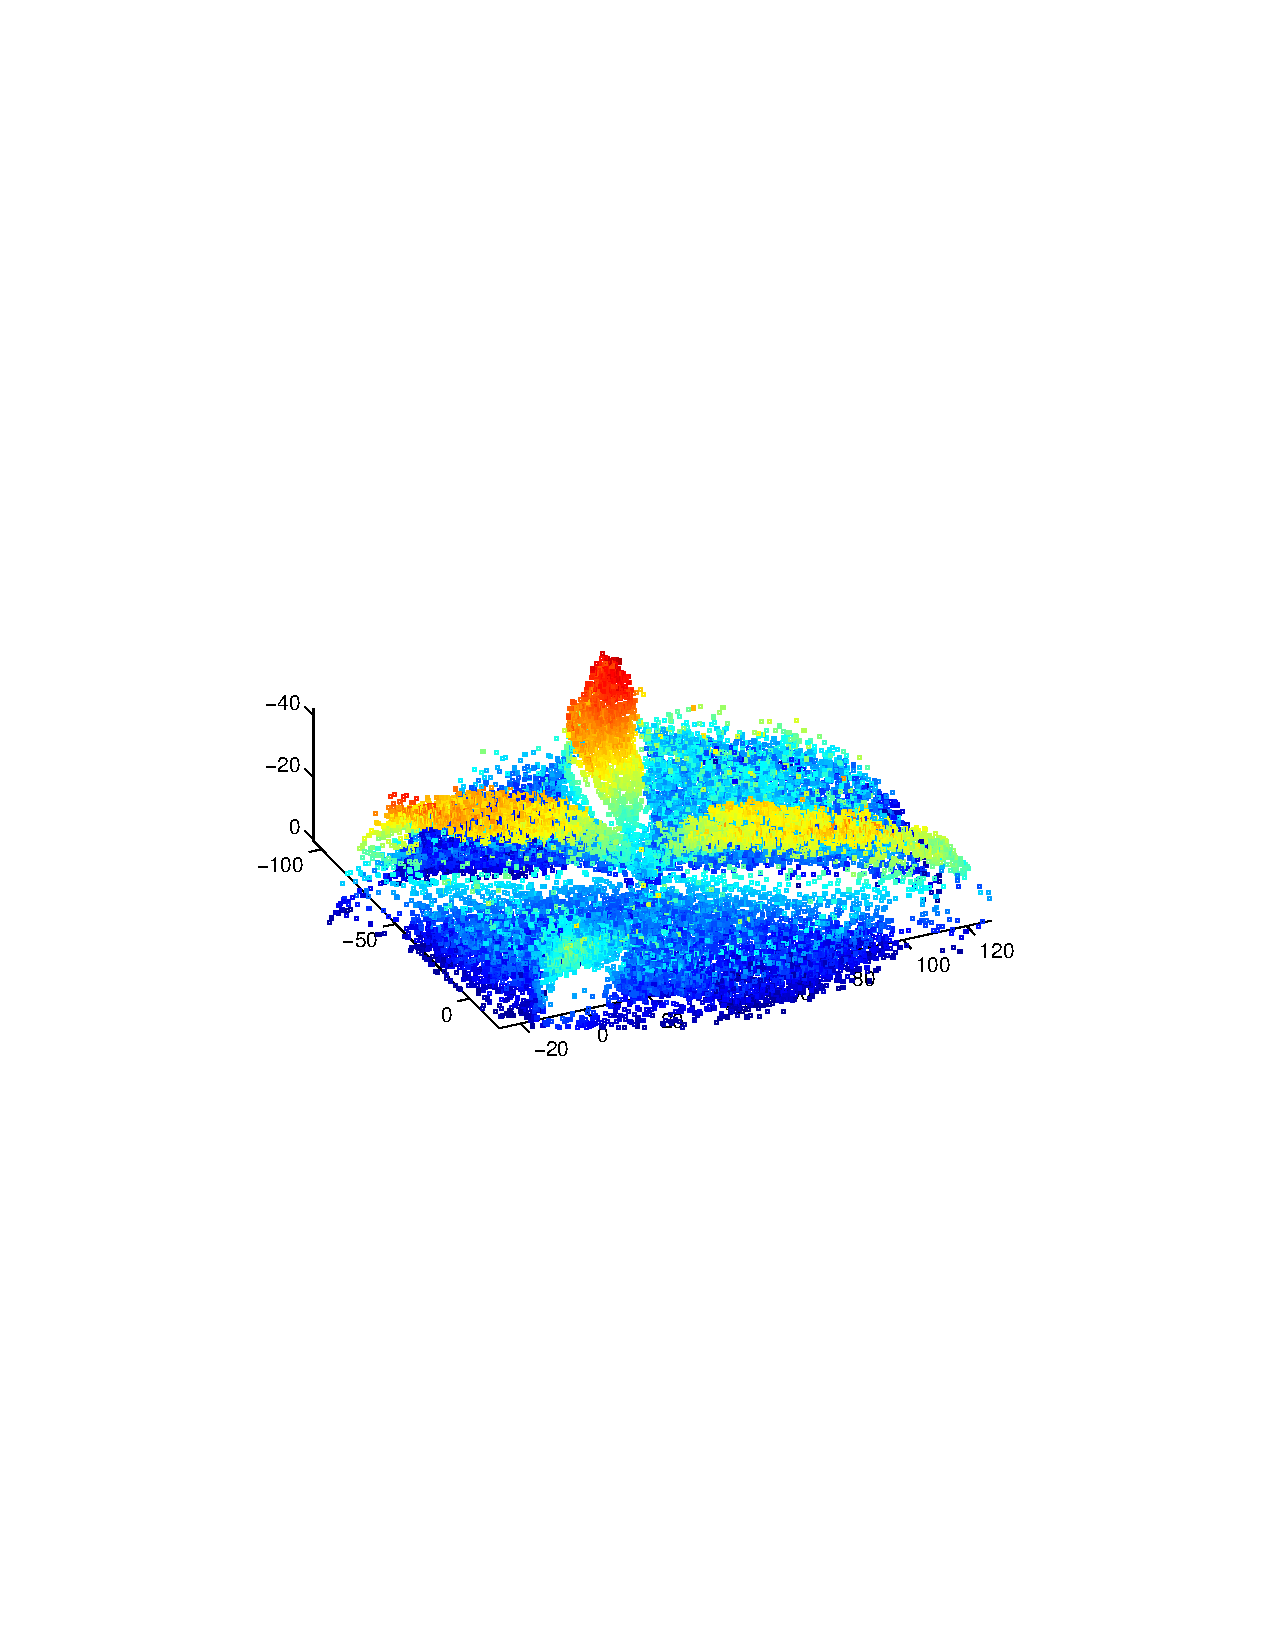
\includegraphics[trim=180 270 180 280,clip,width=0.4\linewidth]{Figures/plant1-noise} &
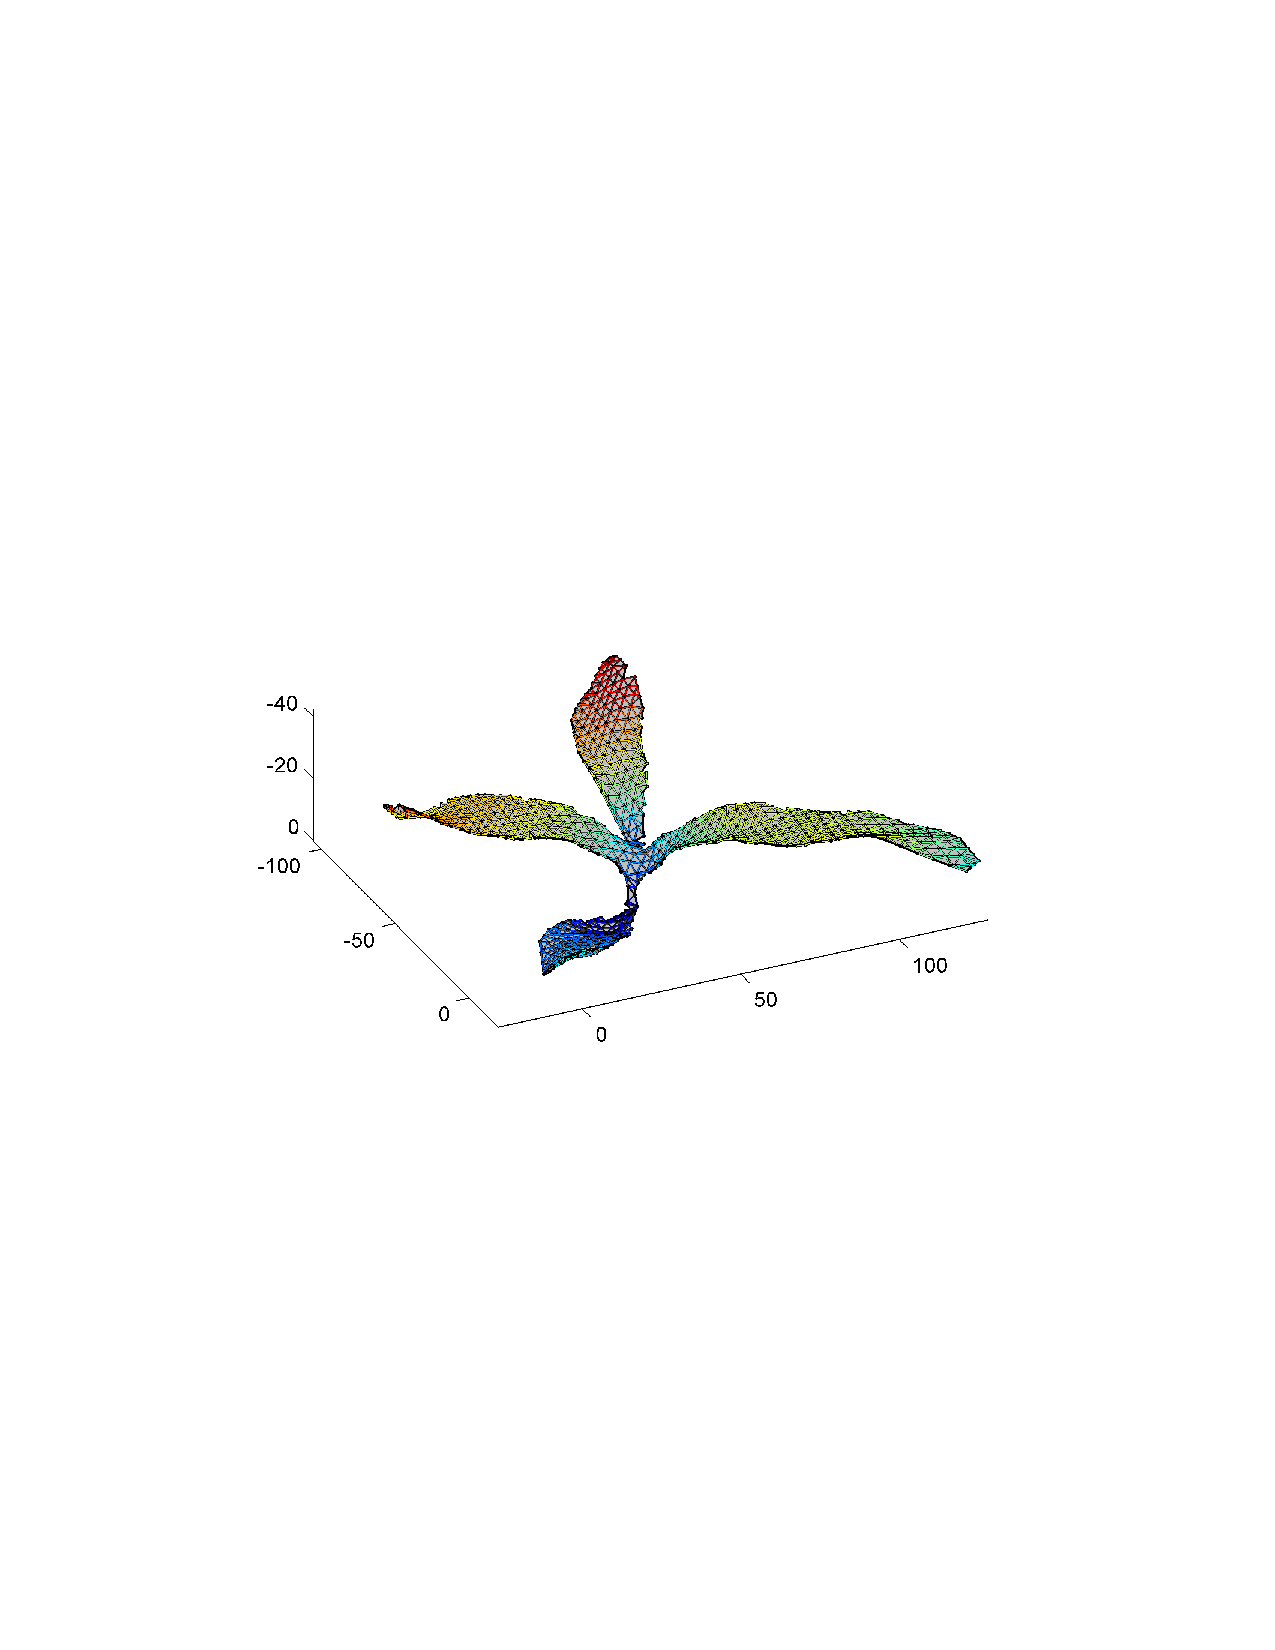
\includegraphics[trim=180 270 180 280,clip,width=0.4\linewidth]{Figures/plant1-mesh} \\
($c$) & ($d$) \\
\end{tabular}
\end{center}
\caption{Illustration of sensor data.  ($a$) Portion of color image. ($b$) IR reflectance image with reflectance values. ($c$) Portion of a single depth image surrounding plant averaged over 60 frames to reduce noise, and projected into $3$D showing significant remaining depth noise. ($d$)  The mesh resulting from the algorithm in this paper using data from the color, depth and IR reflectance images.  Units of $3$D plots are mm.  }
\label{fig:plantnoise}
\end{figure}


An important step in estimating all of the plant phenotypic properties is to obtain $3$D shape and pose for all the plant leaves~\cite{muller2015leaf}, which has to be measured in a limited growth space with minimum disturbance, making it impractical to use scanning lasers for shape modeling. As an alternative, we propose to mount close-range time-of-flight RGB-D sensors in the growth chambers, acquire color, IR-reflectance and range data, and estimate leaf shape through building leaf $3$D mesh models (see Fig.~\ref{fig:plantnoise}). Mesh fitting to $3$D point clouds and depth maps enables visualization and leaf shape analysis by providing a surface topology and geometry to a point cloud~\cite{Sienz2000,Yeh2011}.  A mesh can efficiently compress dense scanned data and mesh fitting methods have been developed that adhere to the underlying shape and preserve geometric features such as creases~\cite{hoppe:1994,Kobbelt:1998}. 
%
However, while time-of-flight RGB-D sensors are small, inexpensive and provide dense $3$D surface sampling of objects, they pose a challenge to surface modeling of small objects due to large depth noise. Specifically, in our leaf $3$D mesh modeling application, the pixel-depth noise has a standard deviation on the order of the surface feature sizes (see Fig.~\ref{fig:sigmainterframe}). In this paper, we present a new solution to automatically build precise $3$D mesh models of plant leaves using time-of-flight RGB-D sensors. We achieve this through formulating an optimization that minimizes depth noise and adds a curvature-based regularization.  

There have been differing goals in previous work on automated $3$D leaf modeling.   One goal has been to generate realistic foliage for graphics~\cite{Bradley:2013}.  Here known leaf shapes are fit to $3$D structure from motion data producing realistic-looking foliage, but not necessarily a close approximation to the actual plant leaf shapes and poses.  In~\cite{Quan:2006} an interactive system enables semi-automatic estimation of complex arrangements of leaves.  



There has been significant work in image-based plant leaf detection and segmentation~\cite{XXX}


%Another goal for mesh fitting is to incrementally build full $3$D models of objects.  Zippered polygons~\cite{Turk1994} builds mesh models from range images and combines them discarding noisy points at the boundaries.  The method developed by Curless and Levoy~\cite{Curless:1996} populates a weighted voxel occupancy grid from the depth data and recovers the surface by triangulating an isosurface.  By raycasting this surface, new camera poses can be aligned and their depths maps contribute to and improve the voxel model.  Advantages of this method include that surface topology is automatically determined, additional data can be readily incorporated, holes can be filled when more data are collected and it incorporates directional uncertainty of range data into the models.  Recent approaches for environment modeling from RGB-D cameras such as Kinect Fusion~\cite{Izadi:2011,Newcombe:2011} build on this voxel modeling and accumulation.  For our application the sensor is fixed and there is no option for merging views from different perspectives.  Artifacts caused by discretization into voxels are significant particularly with high input noise, and the method is limited in incorporating surface smoothness priors. .......MOVE TO RELATED WORK

We propose a new mesh generation algorithm that has the following advantages:
\begin{itemize}
\item It resolves object shape despite large noise in the range images by leveraging multiple sensor modalities.  
\item Edge features of the high resolution color image are used to help select and constrain vertices and mesh edges.  
\item The errors in depth are modeled along camera rays and minimized during fitting to facets.  \item The IR reflectance image is used as a Shape from Shading cue to influence facet surface normals.  
\item A linear least squares solution to Laplacian smoothing is integrated into the mesh fitting for regularization with surface curvature priors, and modification is made to preserve sharp edges and creases.
\end{itemize}





\section{Related Work}
\label{sec:related}



%Optimizing meshes for fit point cloud data has been approached through vertex additions and removals~\cite{Hoppe1994}, although this work assumes the point data are precise and dense.

This work detects and segments plant leaves in color images before fitting a $3$D mesh.  These detection and segmentation tasks can be challenging depending on the clutter, lighting, shadows, overlapping leaves, leaf textures etc., and there have been numerous research efforts in this area to address these challenges.

One class of approaches to leaf segmentation is through combining many low-level features.  Contour detection is well studied although only more recently have they been used for leaf shape and boundary segmentation.  Simple cues like color, texture and local brightness and its combination are extensively used in contour and image boundary detections~\cite{martin2004learning,valliammal2012leaf}. To enhance segmentation and boundary regions, active contours and several improved variants of it~\cite{mishra2011decoupled} are also found to be quite popular in computer vision community. LeafSnap~\cite{kumar2012leafsnap}, a popular mobile application tool that identifies leaf species from photographs of leafs,rely on the more simplistic method of segmenting leaf by estimating the foreground and background color distribution by using Expectation Maximization in the saturation value space of the HSV colorspace. Research has also gained particular attention on segmentation of overlapping leaves for leaf detection. Pape et al.~\cite{Pape2015} tackles the problem of segmenting overlapping leaves partly by thresholding on built 3D histograms cubes of Lab color space both for training and testing data, and the quality of segmentation depends on the homogeneity of training data.

Another class of segmentation methods uses prior models.  Manh et al.~\cite{Manh2001139} use deformable templates in weed leaf segmentation which consists of fitting a parametric models to leaf outlines in image, by minimizing energy term related to internal constraints of the model and salient features of the image, such as color of plant. In related work, Toshev et al.~\cite{toshev2012shape} use both geometric properties of object boundary edges and coherent saliency cues distinct from the background. The method overcomes clutter in realistic scenes by handling segmentation using object specific knowledge like similarity in shape (top-down approach) and region growing principles (bottom up approach) from cues like color texture and normalized perimeter of objects.  

A third approach includes Wei Ma et. al ~\cite{ma2008image} who proposes modeling leaves using voxels. It aims to deal with the highly cluttered background by extracting the more visible apex features (position, middle axis and neighborhood) of the leaves instead of intelligent segmentation, from the volumetric data recovered from the images.  Volumetric data provide pose and position of $3$D leaves, and the $3$D leaf shapes can be extracted from the optimized voxels.

For this paper we restrict ourselves to simplified conditions including non-overlapping leaves, low background clutter, and single plant types.  This is to focus on the task of accurate leaf boundary and surface estimation.  Hence our approach is not to constrain leaf boundaries with prior parametric shape models, but instead rely primarily on color cues for segmentation.




%Another goal for mesh fitting is to incrementally build full $3$D models of objects.  Zippered polygons~\cite{Turk1994} builds mesh models from range images and combines them discarding noisy points at the boundaries.  The method developed by Curless and Levoy~\cite{Curless:1996} populates a weighted voxel occupancy grid from the depth data and recovers the surface by triangulating an isosurface.  By raycasting this surface, new camera poses can be aligned and their depths maps contribute to and improve the voxel model.  Advantages of this method include that surface topology is automatically determined, additional data can be readily incorporated, holes can be filled when more data are collected and it incorporates directional uncertainty of range data into the models.  Recent approaches for environment modeling from RGB-D cameras such as Kinect Fusion~\cite{Izadi:2011,Newcombe:2011} build on this voxel modeling and accumulation.  For our application the sensor is fixed and there is no option for merging views from different perspectives.  Artifacts caused by discretization into voxels are significant particularly with high input noise, and the method is limited in incorporating surface smoothness priors. .......MOVE TO RELATED WORK




\section{Sensor Overview}
\label{sec:overview}

We explore using a new class of RGB-D sensor such as the Creative Senz3D~\cite{nguyen2015vietnamese} to build 3D mesh models of plant leafs. The sensor contains a high resolution color camera ($1280 \times 720$ pixels) adjacent and parallel to a lower resolution depth camera ($320\times240$ pixels).  A flash IR emitter adjacent to these cameras illuminates the scene and depth sensor measures the time-of-travel for the reflected light as well as its reflectance over its pixel grid.  These modalities are illustrated in Figure~\ref{fig:plantnoise}.  Our approach is to leverage of the strengths of each sensor to compensate for weaknesses in the other.  

\subsection{Sensor Issues}

In our application the sensor remains fixed in the growth chamber and so there is not the opportunity to combine measurements from different viewpoints.  Rather, we seek to maximize the information from the different modalities of the sensors.  First leaf outlines can often be more precisely determined in the color camera for three reasons: the color camera has an order of magnitude more pixels than the depth camera, edge pixels in the depth camera are often very noisy due to double reflections, and color is often a useful cue in segmenting leaves.  Thus as in~\cite{Dellen2011} and unlike~\cite{Alenya2011,Alenya2013} low-level segmentation is performed in the full color image.  The color image also provides useful edge cues along leaf creases.

The depth plus reflectance camera can provide leaf pixel cues, albeit at a lower resolution, as well as leaf geometry. Combining these leaf pixel cues with color segments enables automatic selection of the leaf segments.  Then the color boundaries and features can be used to constrain a mesh-based surface fitting of the leaves.

Since we are interested in close-range objects, the baseline separating the color from the depth camera must be accounted for when determining pixel correspondences.  At depth discontinuities, this baseline can result in pixels from two different surfaces, both visible in the depth camera, being projected onto the same pixel region in the color camera.  


Outline:
\begin{enumerate}
\item Depth + IR initial leaf detection
\item Augmented color segmentation
\item Color boundary and edges
\item Mesh fitting and filtering
\end{enumerate}




\label{sec:data}


While the sensor produces dense depth measurements over target leaf surfaces, the noise in depth measurements is significantly larger than the features we are seeking to recover as illustrated in Figure~\ref{fig:plantnoise}($c$).  A key goal in this paper is to overcome this noise to maximize the accuracy of leaf shape estimates.  We start in this section by modeling and quantifying the measurement noise.



\subsection{Noise Characterization}
\label{sec:noise}

Since the depth camera returns an IR reflectance in addition to a depth value at each pixel, both it and the color camera are initially calibrated using Zhang's method~\cite{Zhang2000} to obtain intrinsic and extrinsic parameters.  Thus each pixel in each camera defines a ray from its camera origin.  Depth noise is modeled as a one dimensional random variable, $\varepsilon$, along the ray for each pixel along its ray direction.

The depth noise, $\varepsilon$, is modeled as the sum of an image-varying term, $\varepsilon_I$, and a scene-varying term, $\varepsilon_S$:
\begin{equation}
\varepsilon = \varepsilon_I + \varepsilon_S. \label{eq:epsilon}
\end{equation}
The term $\varepsilon_I$ models the random change in depth for camera pixels of subsequent images of a static scene from a static camera.  To quantify this term we measured the standard deviation $\sigma_I$ in depth of each pixel for a batch of 300 images of a fixed scene containing a flat matte surface.  We repeated this at different poses and depths, and with different surface albedos.  While target depth, inclination, albedo, and pixel position are all correlated with $\sigma_I$, we found that the best predictor for $\sigma_I$ was the IR reflectance intensity, as shown in Figure~\ref{fig:sigmainterframe}.  For typical scenes the single measurement noise in depth is roughly 5mm, although for low reflectivity objects or objects at long range this noise can increase significantly.  Fortunately plant leafs are good IR reflectors.

\begin{figure}
\begin{center}
   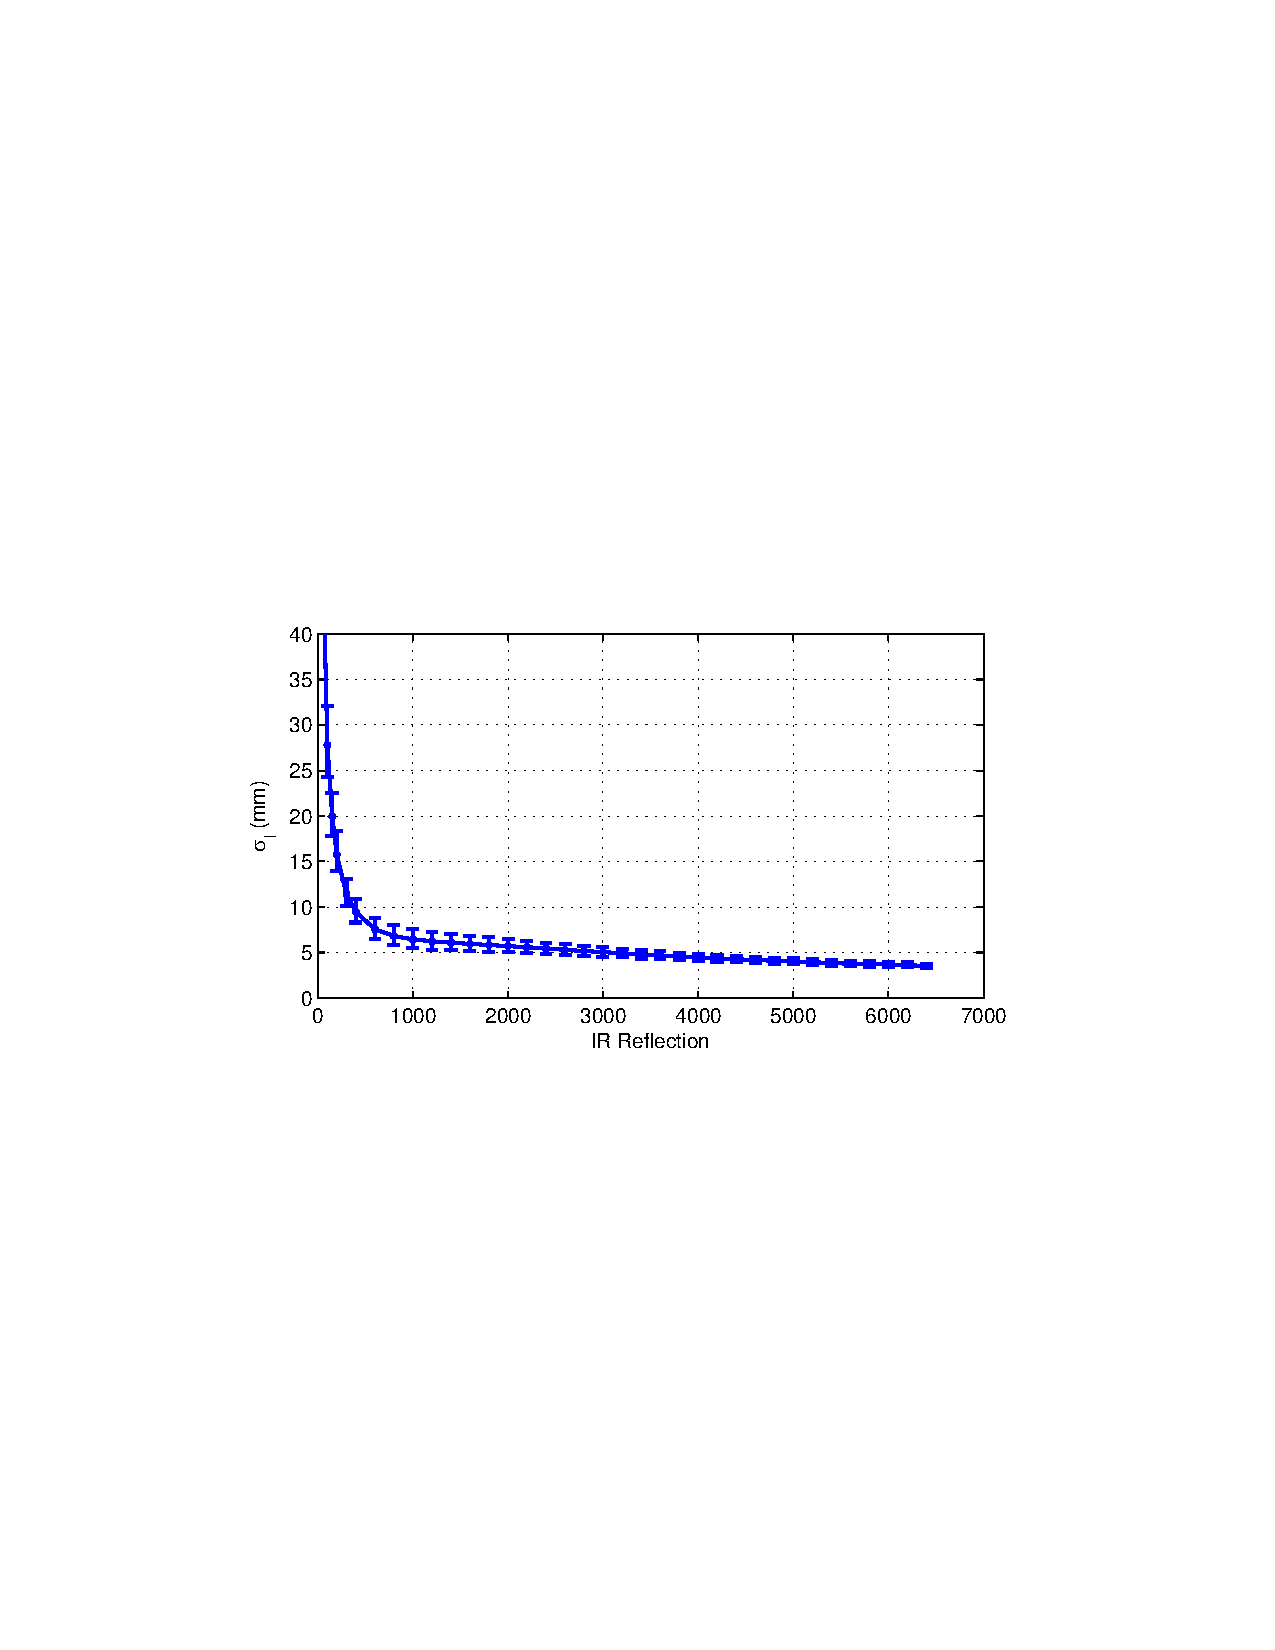
\includegraphics[trim=120 280 110 290,clip,width=0.9\linewidth]{Figures/SigmaInterframe}
\end{center}
   \caption{Image-varying noise, $\sigma_I$, is predicted well by the IR reflectance in raw units returned by the camera, see Figure~\ref{fig:plantnoise}($b$).  The scene-varying noise, $\sigma_S$, is plotted for comparison.}
\label{fig:sigmainterframe}
\end{figure}

Averaging depth measurements of a fixed scene will reduce the noise from $\varepsilon_I$, but will not reduce the noise from $\varepsilon_S$.  This latter scene-varying term is constant for a static scene, but changes when the scene changes.  To characterize this noise we first eliminated (approximately) the image-varying noise contribution by averaging over a large number of images (300).  Then assuming $\varepsilon_S$ is independent and identically distributed between pixels, we measured the variance of the pixel depth errors between a known flat surface and the estimated surface.  In our experiments we obtained $\sigma_S=6.5mm$, and found that it was insensitive to changes in depth.

The total pixel noise can be estimated assuming independence of $\varepsilon_I$ and $\varepsilon_S$, and is given by:
\begin{equation}
\sigma^2 = \frac{\sigma_I^2}{N} + \sigma_S^2,\label{eq:sigma}
\end{equation}
where $N$ is the number of images averaged over.  When averaging 5 or more depth images the scene-varying contribution, $\sigma_S^2$, will dominate.  There are additional sources of noise not modeled by this.  These include object specularities, and mixed-depth pixels on object edges.  These tend to produce very large image-varying noise, $\sigma_I$, and we can filter these points by discarding depth pixels with $\sigma_I>20$mm.  

\subsection{Occlusion Modeling}


\begin{figure}
\begin{center}
   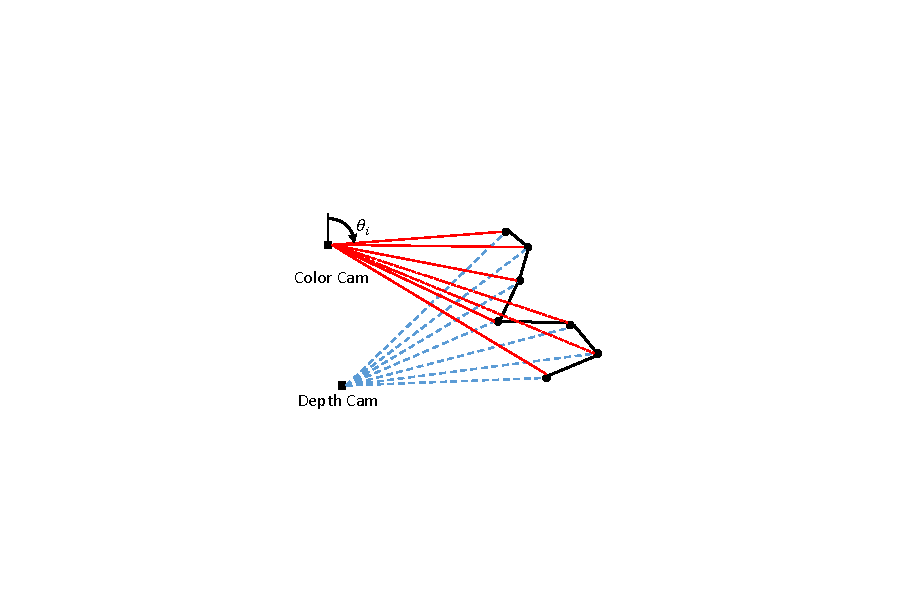
\includegraphics[trim=130 90 140 90,clip,width=0.75\linewidth]{Figures/OcclusionModeling}
\end{center}
   \caption{Occlusion modeling }
\label{fig:occlusion}
\end{figure}


\begin{figure}
\begin{center}
\begin{tabular}{cc}
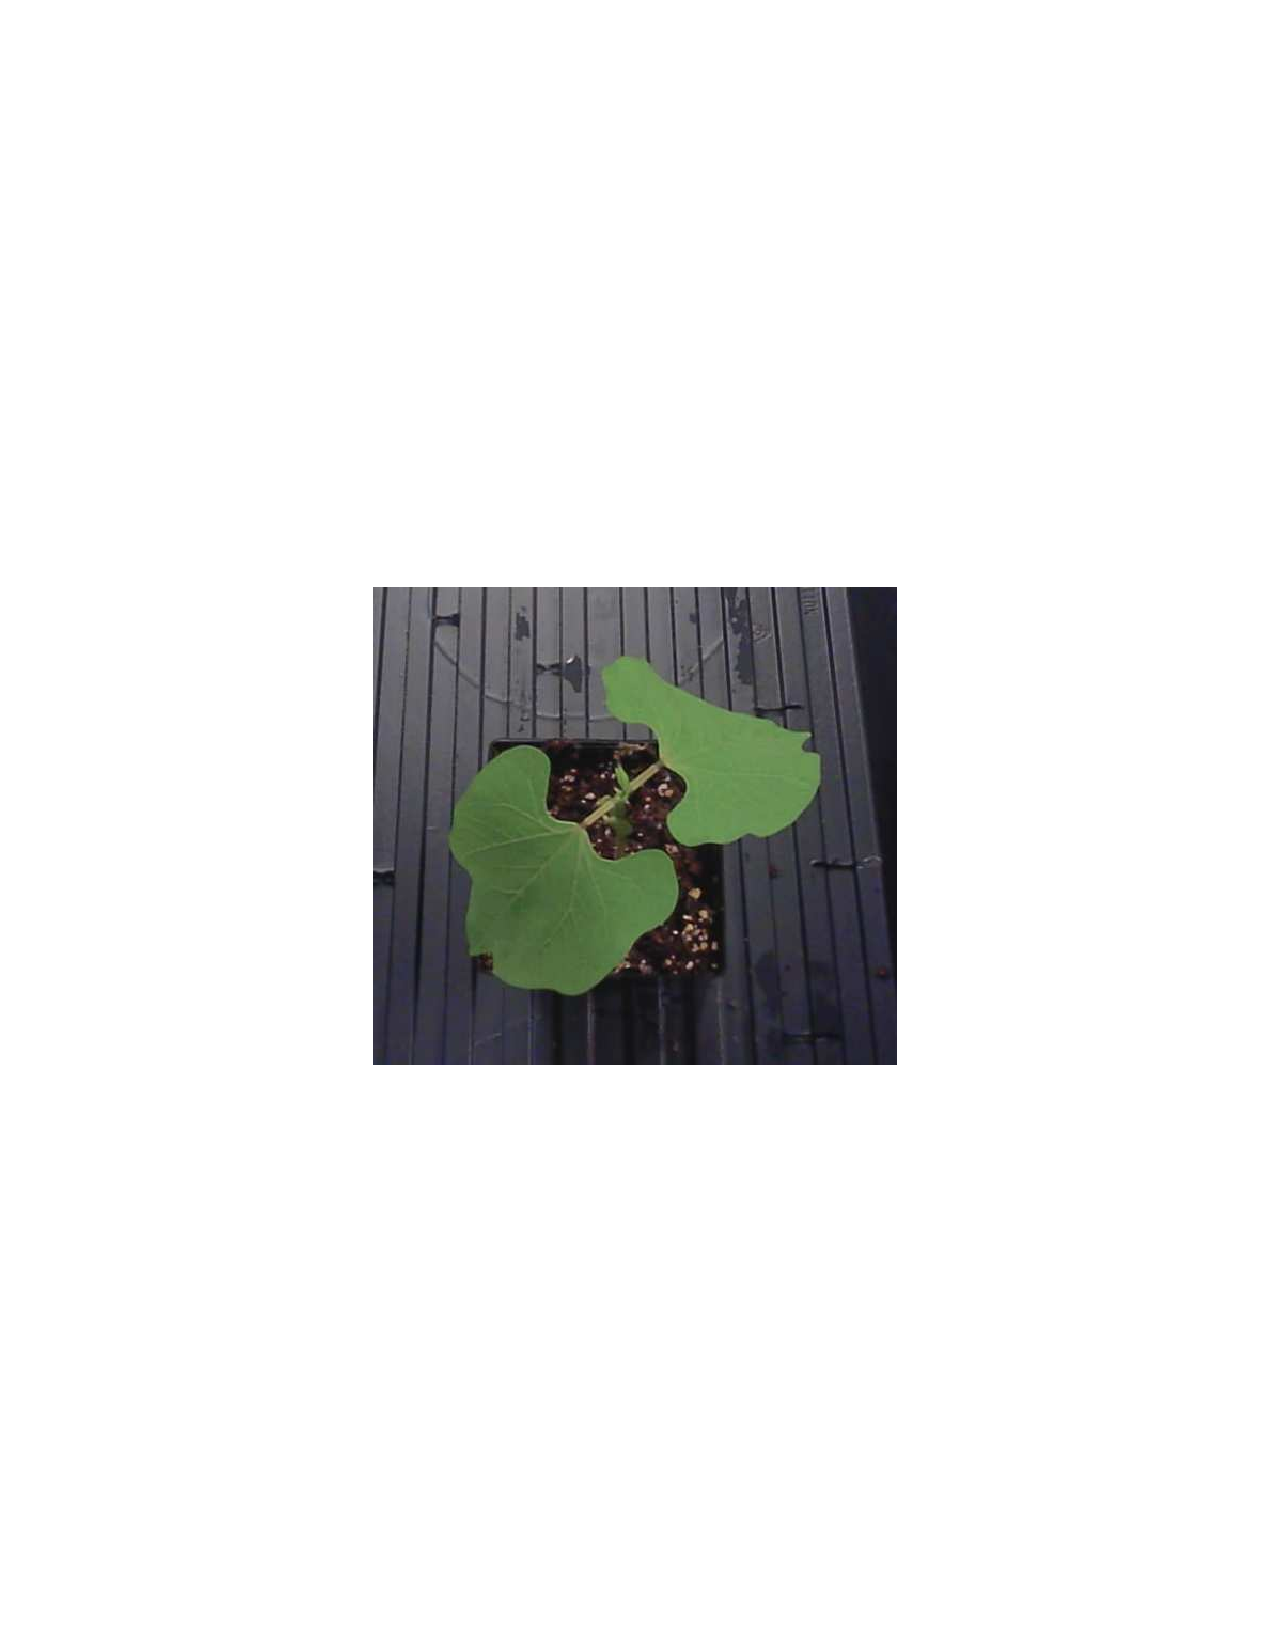
\includegraphics[trim=190 280 190 290,clip,width=0.48\linewidth]{Figures/beanColor} &
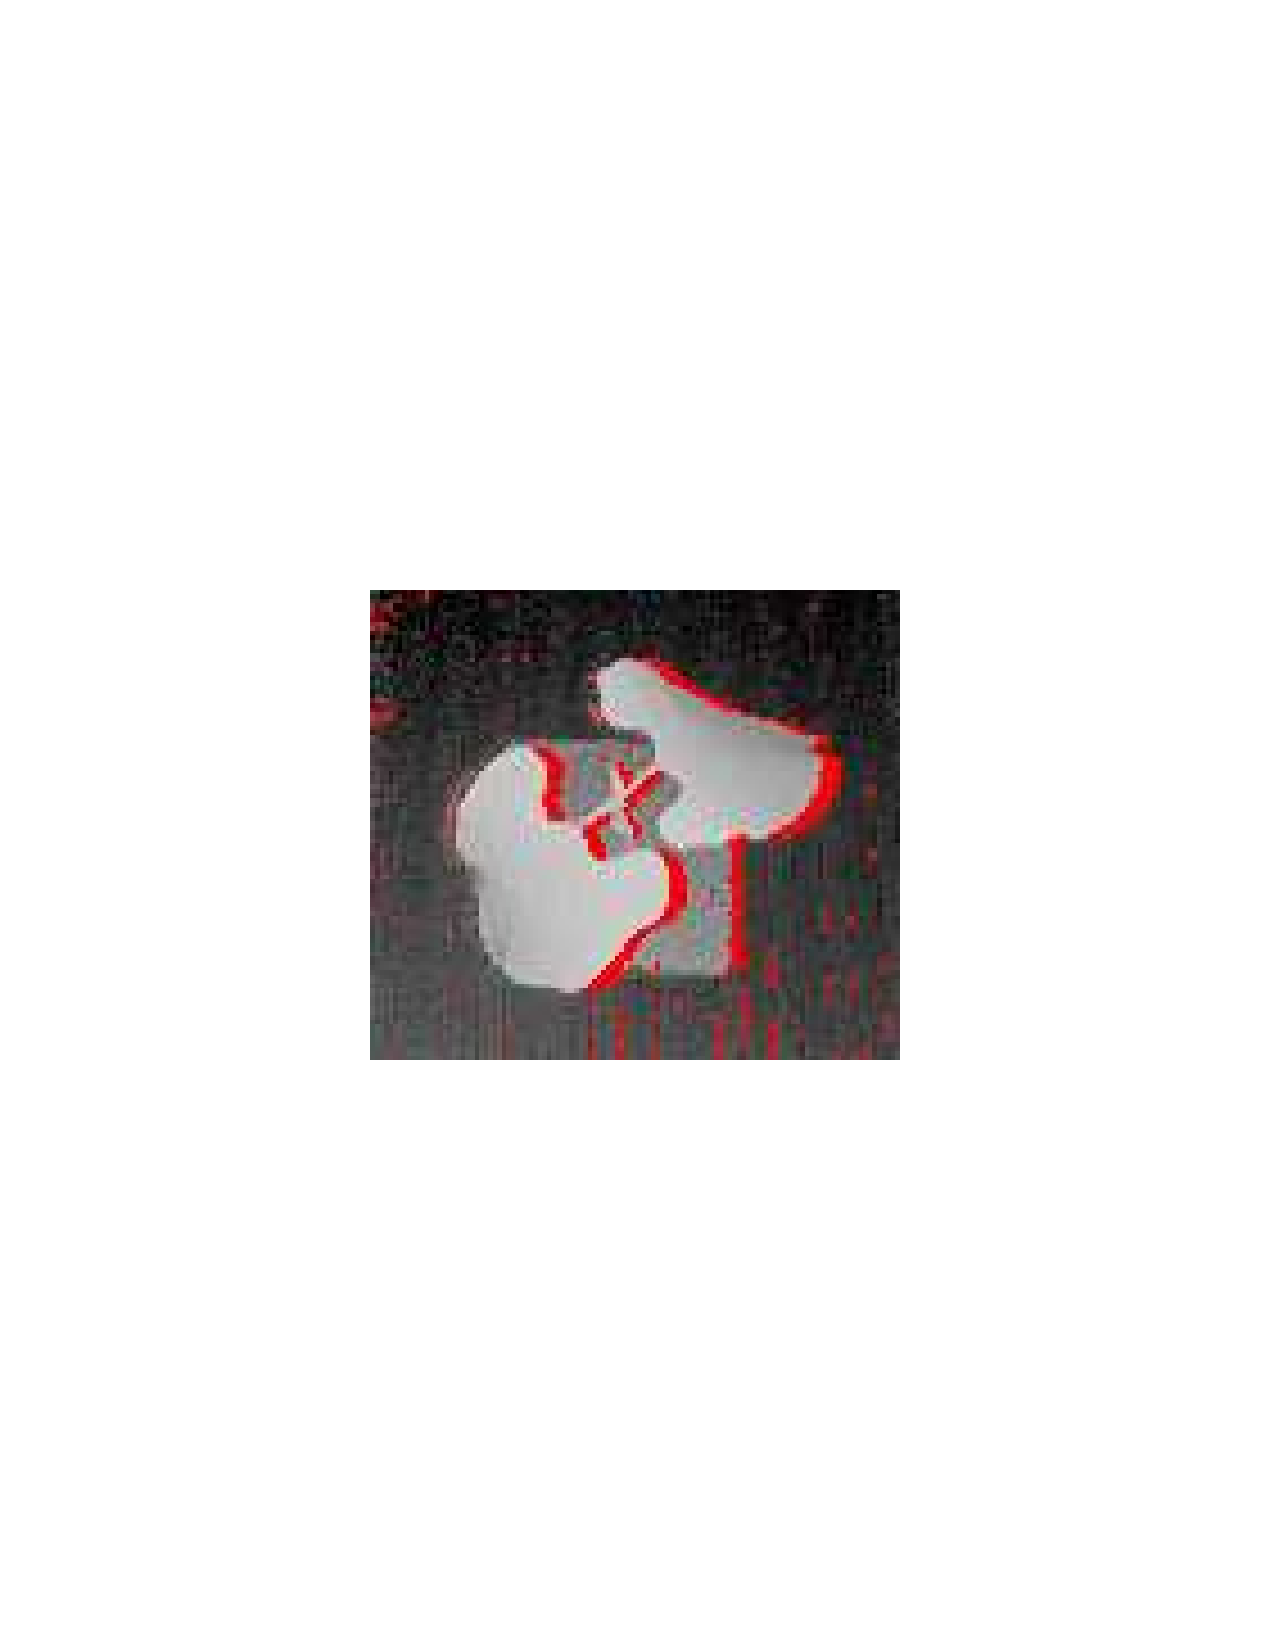
\includegraphics[trim=190 280 190 290,clip,width=0.48\linewidth]{Figures/beanDepth} \\
($a$) & ($b$) \\
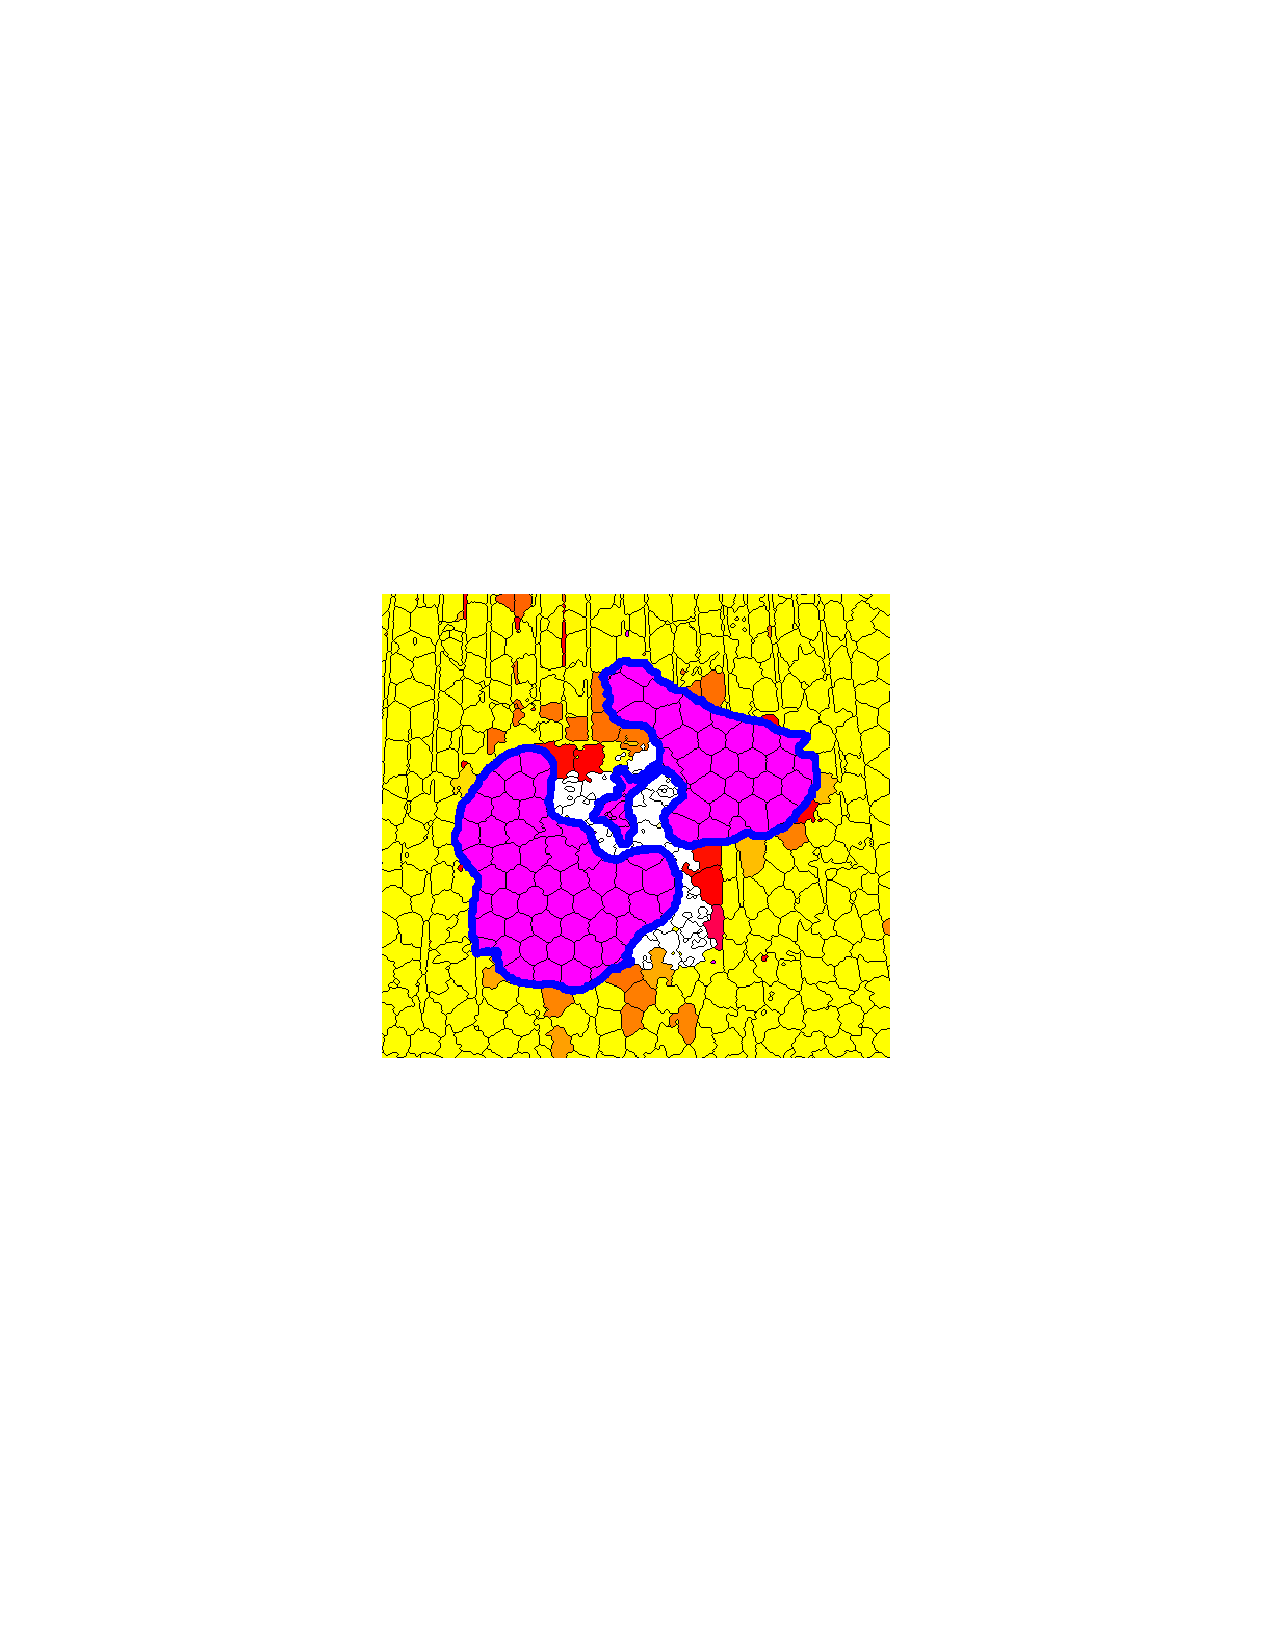
\includegraphics[trim=80 170 80 140,clip,width=0.48\linewidth]{Figures/slic_cropped2} &
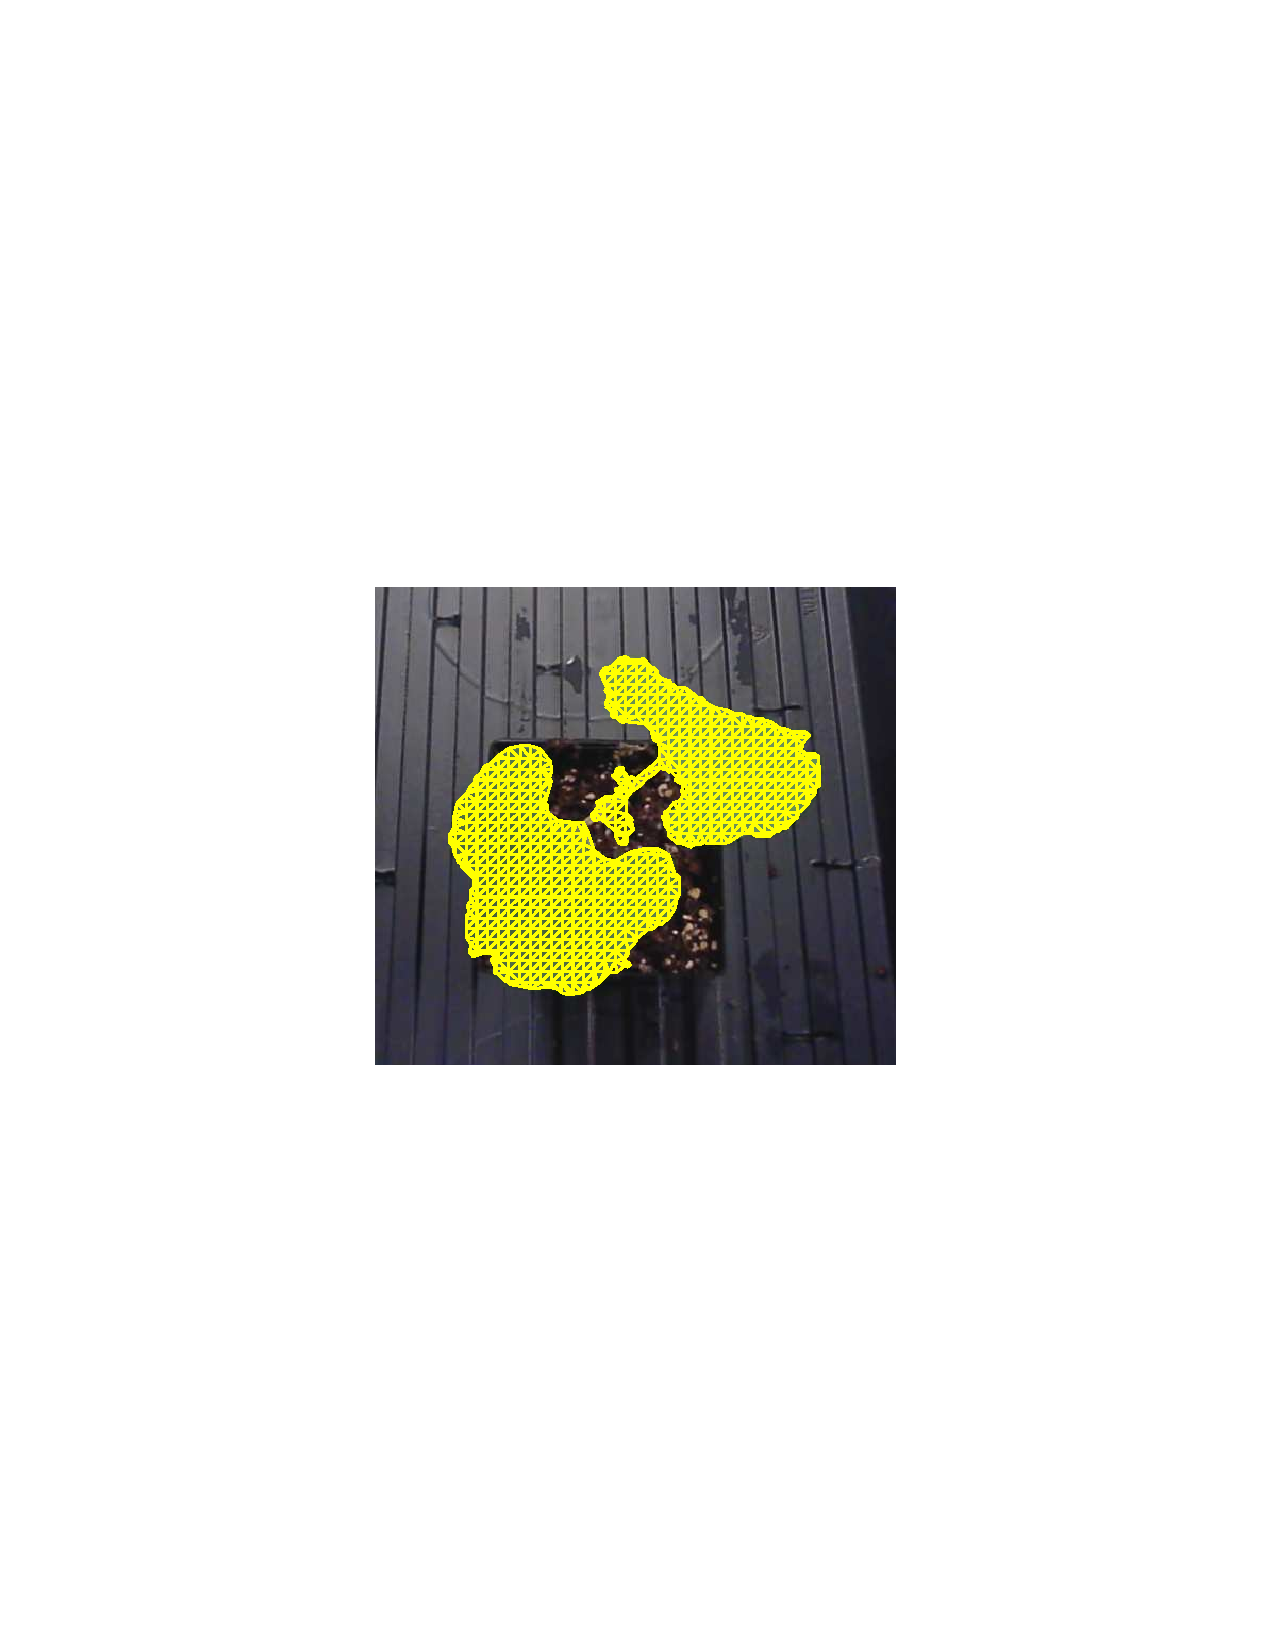
\includegraphics[trim=190 280 190 290,clip,width=0.48\linewidth]{Figures/beanColorMesh} \\
($c$) & ($d$) \\
\end{tabular}
\end{center}
\caption{Initial algorithm steps.  ($a$) Color image portion on plant.  ($b$) Depth image, where red pixels are those that are masked out using the method in Fig.~\ref{fig:occlusion} as they are not visible in the color image. ($c$) SLIC superpixels on LAB color space.Each of the superpixels are colored with the mean L, a and b values of that particular superpixel. The leaf boundaries obtained by integrating the superpixels having the leaf pigments are shown in green dots. ($d$) An mesh is defined in the color image with evenly spaced vertices within and along the leaf boundaries. }
\label{fig:beanimageprocess}
\end{figure}



\section{Color-Based Mesh Cues}
\label{sec:colormesh}

Since we do not deal with overlapping and highly cluttered background, the segmentation can be done easily by using the color information of the rgb image. The initial segmentation on the leaf is done by using the K-means cluster on the �a� and �b� channels of the Lab color space. It is found that the �a� and �b� channels contain much better information about the green pigments of the leaf. Using only three clusters on these two channels in the k-means clustering, it is able to give a rough mask of where the leaf regions are. But for an accurate mesh fitting, it is required to find the leaf shape by following the edges of the shape boundaries as closely as possible. It is well known in the literature that superpixels ~\cite{achanta2012slic} can split image into multiple homogenous regions and adhere shape boundaries very closely. We use the simple linear iterative clustering (SLIC) superpixels to form superpixels on the entire image. It is found that though SLIC superpixels form an oversegmentation of the image, they are found to adhere very closely to the leaf boundaries. To detect whether each superpixel belongs to the leaf pigments or not, the initial batch of superpixels are selected by computing the centroid of each of them and checking whether it falls within the initial mask developed by K-means cluster. Any non leaf superpixels that are chosen in the first selection are then filtered out by thresholding on the ratio of 'a' and 'b' channels of the Lab color space. The selected superpixels are then merged to create the segmented plant/leaf segment.

We build line segment based on boundary pixels of the segmented plant/leaf boundaries. Since plant leaves are clumped together in a single structure, it is possible to get closed boundary on the entire segmented image of the plant. We then perform a polygonal approximation motivated by the merging technique ~\cite{Leu1988231} process on the boundary by approximating straight lines with a maximum deviation of one pixels from pixels in the original boundary ~\cite{KovesiMATLABCode}. The two end points of the approximated lines are saved as vertices that join an edge of the polygon.

Having obtained the polygonal approximation of the plant leaf boundaries, we then sample points with a uniform spacing of $\ell$ pixels on each side of the polygon. Uniform grid of points with a spacing of $r$ are also created in the entire image, and the grid points which fall within or on the mask structure are only selected. Points falling within $\ell \leq r$ are removed from the set of selected grid points. Both the selected grid points and the sampled points on the boundary are then used to create a delaunay triangulation on the plant mask.The slivers of triangular facets that lie outside the polygonal shape are removed by seeking whether the midpoints of the line fall within the polygonal shape or not.The final meshes on a typical rgb plant image looks like in Figure~\ref{fig:mesh}:

\begin{figure}[!t]
  \vspace{-20pt}
  \centering
  % Requires \usepackage{graphicx}
  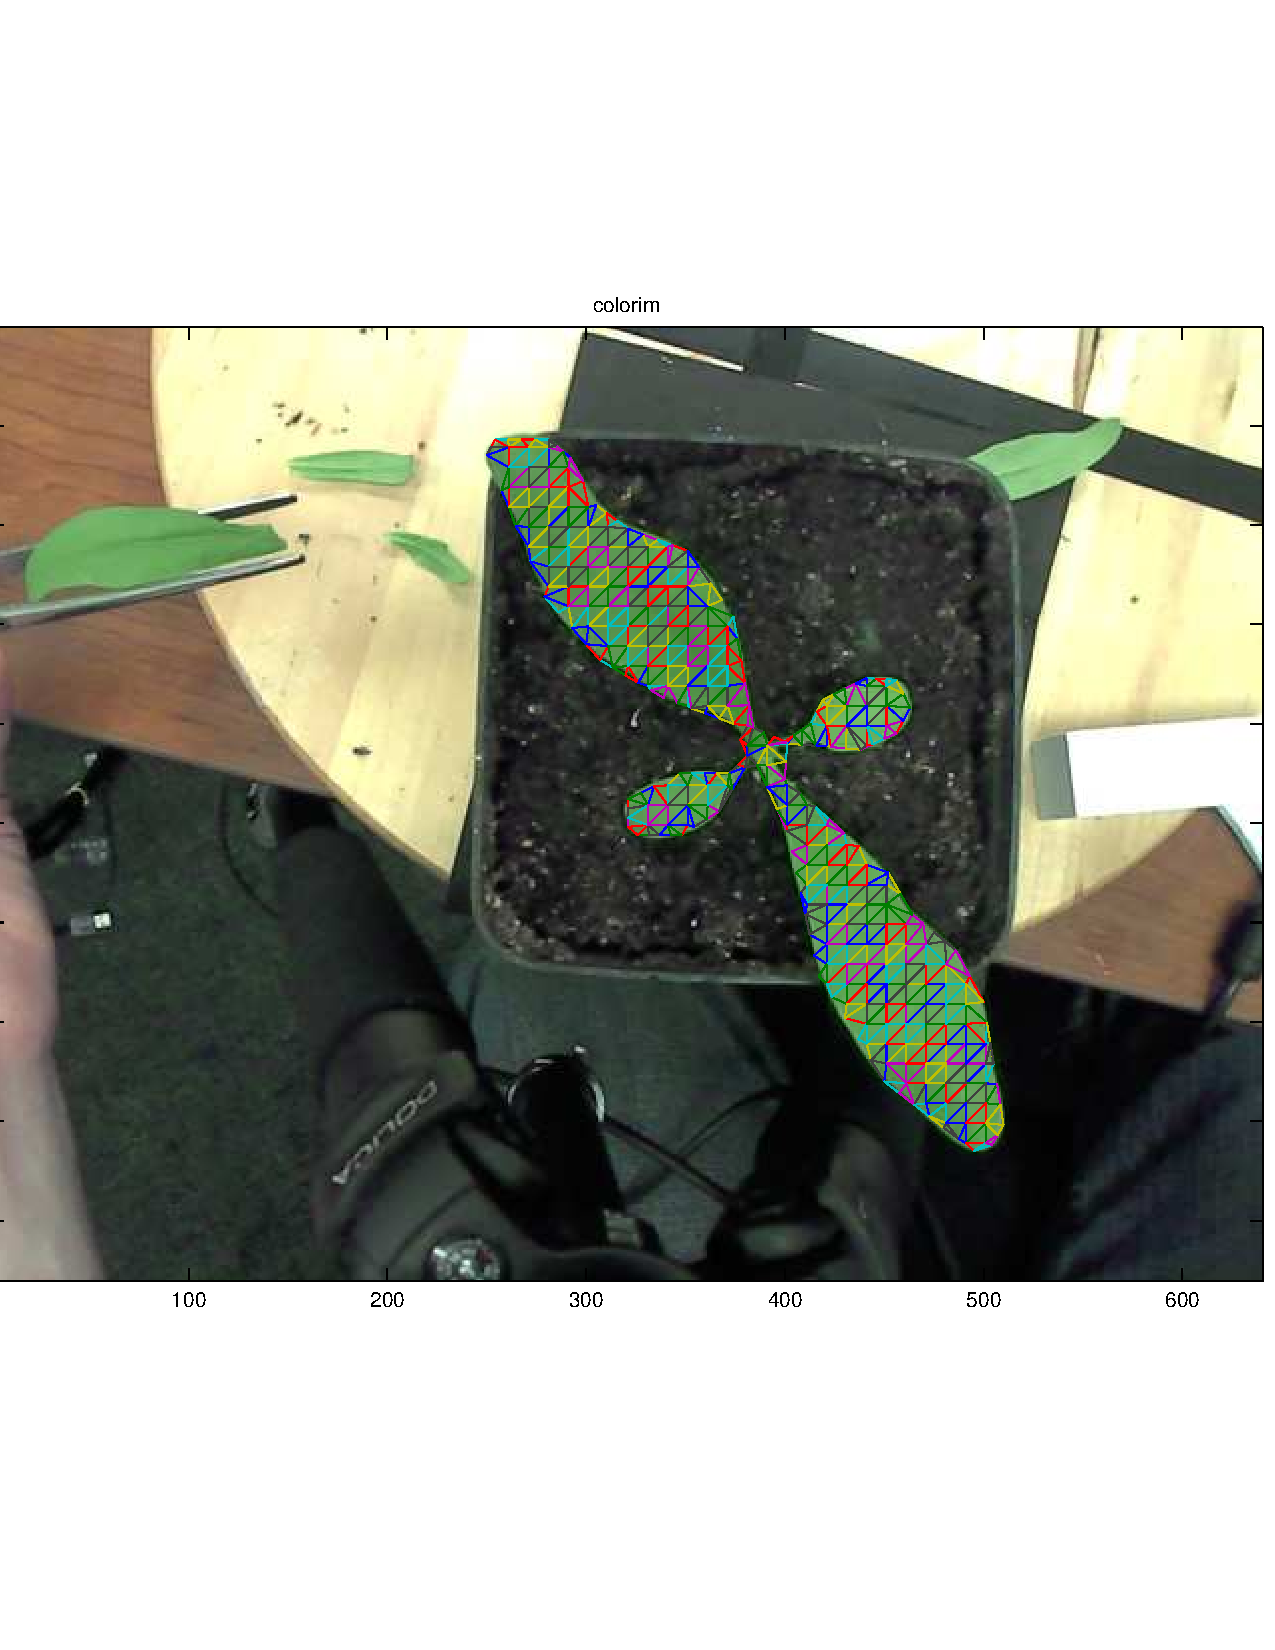
\includegraphics[trim=150 180 120 120,clip,width=0.6\linewidth]{Figures/meshonplant}\\
  \caption{Mesh Distribution on the RGB Plant Imagery}\label{fig:mesh}
\end{figure}



\section{Mesh Fitting}
\label{sec:fitting}

We pose mesh fitting to 3D point data as finding the most likely surface that would have generated those points.  By incorporating prior surface assumptions, the fitting process estimates a continuous surface from discrete points that can eliminate much of the measurement noise.  Methods that fit mesh models to 3D points often minimize the perpendicular distance of points to facets [REF].  This makes sense when point-cloud noise is equal in all directions or else the point noise is small compared to the facets.  For our data the measurement noise is large and is not equal in all directions, but rather is along the depth camera rays.  Hence the focus of this section is to develop a mesh fitting method that minimizes these pixel depth errors along the pixel rays.

In this paper we define a mesh in a $2$D image space and project it into $3$D.  This is more limiting than full $3$D meshes as it models only the surface portions visible from the sensor, but it also provides a number of advantages.  Compared to methods that fit prior surface models to depth maps [ref], need to search of the space of poses, scales and distortions of the model with the chance of finding local minima.  Compared to voxel-based models with implicit surfaces [ref], our method can better incorporate pixels uncertainties and surface priors, as well as having fewer discretization artifacts.  In addition our method can naturally incorporate detailed features from the high-resolution color camera, and reflectivity information from the IR reflectance image.

\subsection{Notation}

A vertex, $\vertex$, is a vector in $3$D.  In a given camera coordinate system, it projects onto a pixel on the unit focal-length image-plane $\hvertex=(u,v,1)^\top$, where the `` $\tilde{\text{ }}$ '' indicates a homogeneous vector, and $u$ and $v$ are the coordinates in this plane.  Now $\hvertex$ defines a ray from the camera origin, and the original vertex is obtained by scaling the image-plane vertex by its depth, $\lambda$, along the ray, namely: $\vertex = \lambda\hvertex$. 

\subsection{Facet Model}

Mesh fitting for an individual facet is illustrated in Figure~\ref{fig:facet}.  The $2$D vertices and edge connections are determined in an image, in this case the color image although it could be the depth image, as described in section~\ref{sec:mesh}.  If these vertices lie on a feature of the target leaf, such as its edge, we know that that those $3$D features like somewhere along the rays emanating from camera origin through those vertices.  Hence a triangular facet approximation to the object surface will have vertices on these three rays.  

\begin{figure}
\begin{center}
   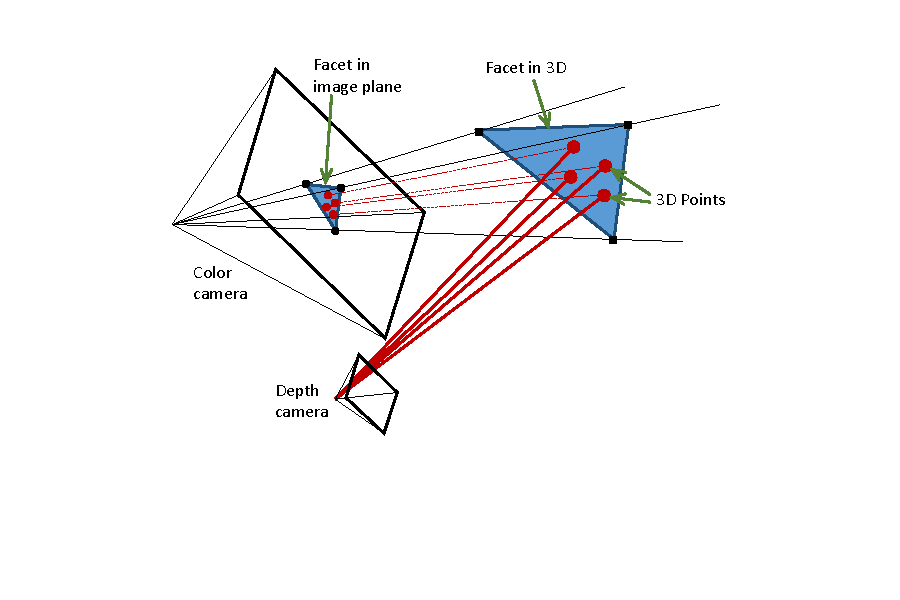
\includegraphics[trim=80 70 70 20,clip,width=0.95\linewidth]{Figures/pointFittingConcept}
\end{center}
   \caption{The parallel and adjacent color and depth cameras are shown as pyramids denoting their fields of view, and their size difference illustrates their relative resolutions.  Three vertices in a color image define the rays on which the vertices of the corresponding $3$D object facet must lie.  This facet is fit using the the $3$D points projected out from the depth camera.}
\label{fig:facet}
\end{figure}

The next step is to associate depth measurements with the facet.  Pixels in the depth camera are projected along their rays out into $3$D.  The resulting $3$D points that lie within the facet pyramid (defined by these rays through its vertices) will project into the $2$D facet in the color image.  Hence it is straightforward to associate $3$D points with mesh facets.  

To estimate the facet parameters from depth measurements we will express the depth points as a linear function of the vertices of its facet.  We make a local orthographic approximation for the projection of a facet.  This will be a good approximation as long as the facet size is small compared to is depth from the camera, which is true for most applications.  Given this assumption, the coordinates of a point $\point$ lying on a facet can be expressed as a linear combination of the three vertex coordinates $\vertex_a$, $\vertex_b$ and $\vertex_c$ as follows:
\beq  %see PlantMacros.tex
\point = \alpha_a \vertex_a + \alpha_b \vertex_b + \alpha_c \vertex_c. \label{eq:point}
\eeq
The coefficients $\alpha_a$, $\alpha_b$ and $\alpha_c$ are defined in Figure~\ref{fig:triangle}.  Substituting in depth-scaled homogeneous vectors, and taking the third row, we obtain an equation for the point depth, $\lambda_{p}$:
\beq
\lambda_{p} = \alpha_a \lambda_a + \alpha_b \lambda_b + \alpha_c \lambda_c, \label{eq:pointdepth}
\eeq
where $\lambda_a$ is the depth of $\vertex_a$ and so forth.  

\begin{figure}
\begin{center}
   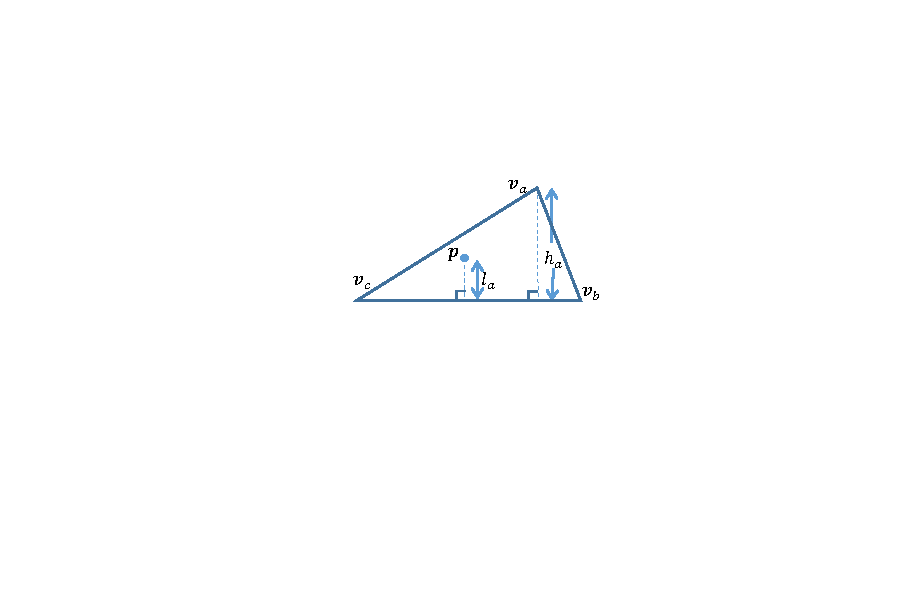
\includegraphics[trim=150 140 140 80,clip,width=0.75\linewidth]{Figures/TriangleParameterization}
\end{center}
   \caption{The coordinates of a point on a facet described by Eq.~(\ref{eq:point}) are the weighted linear sum of the three vertex coordinates.  The weight, $\alpha_a$, for vertex $\vertex_a$ is given by $\alpha_a = \frac{l_a}{h_a}$, the ratio of its perpendicular distance $l_a$ to the opposite edge to the vertex perpendicular distance $h_a$.  Analogous expressions describe $\alpha_b$ and $\alpha_c$. }
\label{fig:triangle}
\end{figure}

\subsection{Least Squares Depth}

Equation (\ref{eq:pointdepth}) gives the depth of one point in terms of its facet vertices.  For mesh with many facets and a measurement with many depth points, a vector of pixel depths, $\vlambda_d$, and vector of vertex depths, $\vlambda_v$, are related with a coefficient matrix, $A$, containing the appropriate $\alpha$'s:
\beq
\vlambda_d = A \vlambda_v. \label{eq:linearmesh}
\eeq
Given a measurement vector of point depths, $\bar{\vlambda}_d$, expressed in the color camera coordinates, the error vector between these depths and the corresponding mesh points is: $\bar{\vlambda}_d - A \vlambda_v$.  Notice that this error is along the color camera rays which to a good approximation are parallel to the depth camera rays, and thus the noise model in Eq.~(\ref{eq:sigma}) applies.  This justifies the following weighted squared error formulation:
\beq
E_{depth} = \| W \bar{\vlambda}_d - W A \vlambda_v \|^2, \label{eq:meshleastsquares}
\eeq
where $W$ is a diagonal matrix containing the inverse standard deviation, $\sigma^{-1}$, from Eq.~(\ref{eq:sigma}).

\subsection{Shape from Shading}

The depth camera measures IR reflectance in addition to depth at each pixel.  Since the reflectance depends on the angle between the surface normal and the incident ray from the IR illuminator, the reflectance image can provide useful cues on the object surface.  Shape from shading techniques model this dependence on the surface normal, along with additional surface assumptions such as smoothness, to estimate the normals and integrate an object surface [REF].  However the real world practicality of these methods has been limited since they generally require a single known light source position illuminating a Lambertian surface, the integration is sensitive to noise, and shape is obtained only up to a scale factor.  Fortunately our application satisfies the key requirements of Shape from Shading, (we have a known light source and leafs are modeled well as Lambertian surfaces~\cite{Chelle2006219}), and our mesh model provides additional information that removes the need to integrate noisy surface normals.  This section describes our use of Shape from Shading to improve shape recovery.

\begin{figure}
\begin{center}
   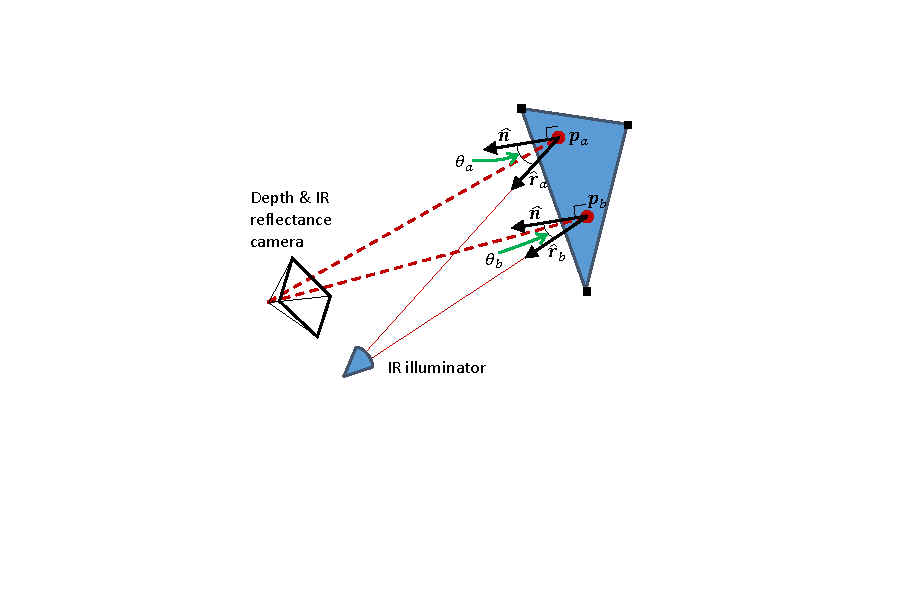
\includegraphics[trim=100 100 100 40,clip,width=0.95\linewidth]{Figures/ShapeFromShading}
\end{center}
   \caption{Our geometric model for the reflectance image.  At each depth point the intensity of the reflectance image will depend on a number of factors including the angle between the facet normal and the ray to the illuminator shown for two points as $\theta_a$ and $\theta_b$. }
\label{fig:shapefromshading}
\end{figure}

\subsubsection{Reflectance Modeling}

We build a simplified bidirectional reflectance model to explain the pixel values, $R_i$, of the IR reflectance image, shown in Figure~\ref{fig:plantnoise}($b$).  This model for pixel $i$ is:
\beq
R_i = \frac{I_i}{r_i^h}\ray_i\cdot\normal_i \rho s_i.\label{eq:reflectanceinit}
\eeq
Here $I_i$ is the intensity of the ray from the IR illuminator.  For a source emanating in all directions this would decrease with a factor of $\frac{1}{r_i^2}$, but a focused beam the decrease may be less, and we model the decay power with $h$.  Under a Lambertian assumption the reflected beam is given by $\ray_i\dot\normal_i \rho = \cos(\theta_i) \rho$ where $\theta_i$ is the angle between the ray to source $\ray_i$ and the surface normal $\normal_i$, and $\rho$ is the albedo.  Finally the sensor scales the incoming beam with a factor $s_i$.  This model can be simplified further by merging some of the unknown parameters.  We define a pixel gain $g_i = \log(I_i \rho s_i)$, and the resulting model is:
\beq
R_i = \frac{ \exp(g_i) \cos(\theta_i)}{r_i^h}. \label{eq:reflectance}
\eeq

The unknown parameters in Eq.~\ref{eq:reflectance} are $g_i$ and $h$, and they can be calibrated as follows.   Depth and reflectance images are taken of a flat, uniform albedo target at various depths and inclinations.  




\subsection{Regularization}

Prior models on surface properties can be incorporated into the mesh via regularization and in so doing reduce the impact of noise.  Membrane energy is a well-used function in mesh optimization~\cite{Kobbelt:1998} and can be minimized using the discrete Laplacian operator.  Here we use Laplacian smoothing due to its simplicity and good performance~\cite{Kobbelt:1998,Ohtake2001789,Chen2005376}, although we modify it to accommodate image-based edge information.  In addition, rather than apply Laplacian smoothing after the fact, entailing an iterative optimization~\cite{Kobbelt:1998}, we show that Laplacian smoothing can be incorporated directly into the least squares mesh estimation.  This has a number of  advantages over application after the initial mesh estimation.  First the smoothing penalty is traded off against measurement error rather than vertex offset.  Second, the due to our ray constraints on the vertices we are able to derive a linear solution with not need to iterate.  Finally  when the regularization components are added to Eq.~(\ref{eq:meshleastsquares}) they ensure that the solution is well-posed even when some of the facets have no depth points in them.

Laplacian smoothing uses an umbrella-operator~\cite{Kobbelt:1998} on a vertex, $\vertex$, and its neighbors $\vertex_i\in\mathcal{N}(\vertex)$,
\beq
\vect{u}(\vertex) = \frac{1}{n}\sum_{\vertex_i\in\mathcal{N}} \vertex_i - \vertex,\label{eq:umbrella}
\eeq
for $n$ neighbors as illustrated in Figure~\ref{fig:laplacian}.  In our model the vertices lie along known rays and so this operator can be expressed as a function of the vertex depth: $\vect{u}(\lambda) = \frac{1}{n}\sum_{i\in\mathcal{N}} \lambda_i \hvertex_i - \lambda\hvertex$.  The squared magnitude $\|\vect{u}(\lambda)\|^2$ is a natural penalty term as it captures a discrete form of the membrane energy.  Summing this over all vertices and arranging the known $\hvertex$ components into a single matrix $U$, we obtain
\beq
E_{reg} = \| U \vlambda \|^2.
\eeq

\begin{figure}
\begin{center}
   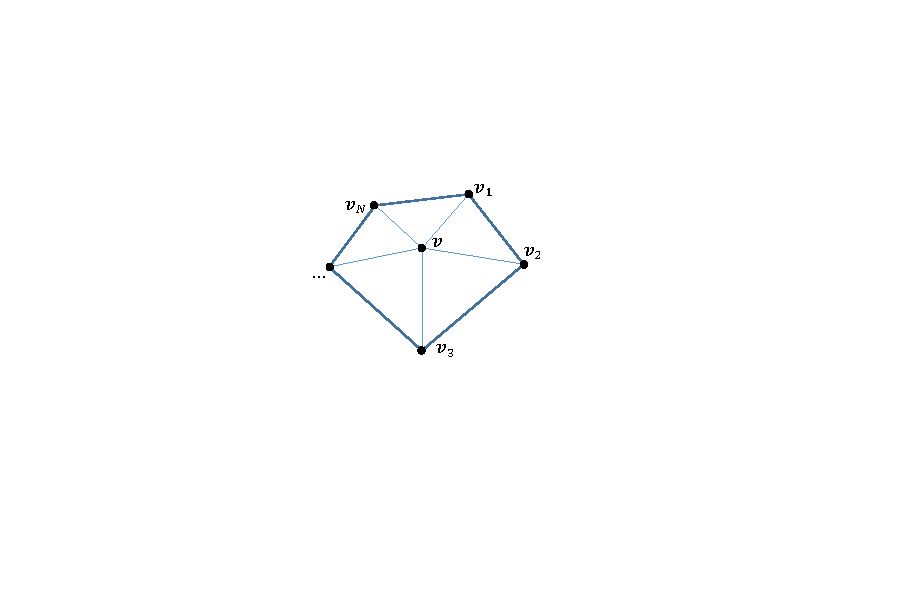
\includegraphics[trim=100 110 140 90,clip,width=0.8\linewidth]{Figures/LaplacianFacets}
\end{center}
   \caption{In discrete form the Laplacing is implemented as an umbrella operator, Eq.~(\ref{eq:umbrella}), over a vertex $\vertex$ and its first neighbors.}
\label{fig:laplacian}
\end{figure}




\section{Results}
\label{sec:results}


\begin{figure}
\begin{center}
\begin{tabular}{cc}
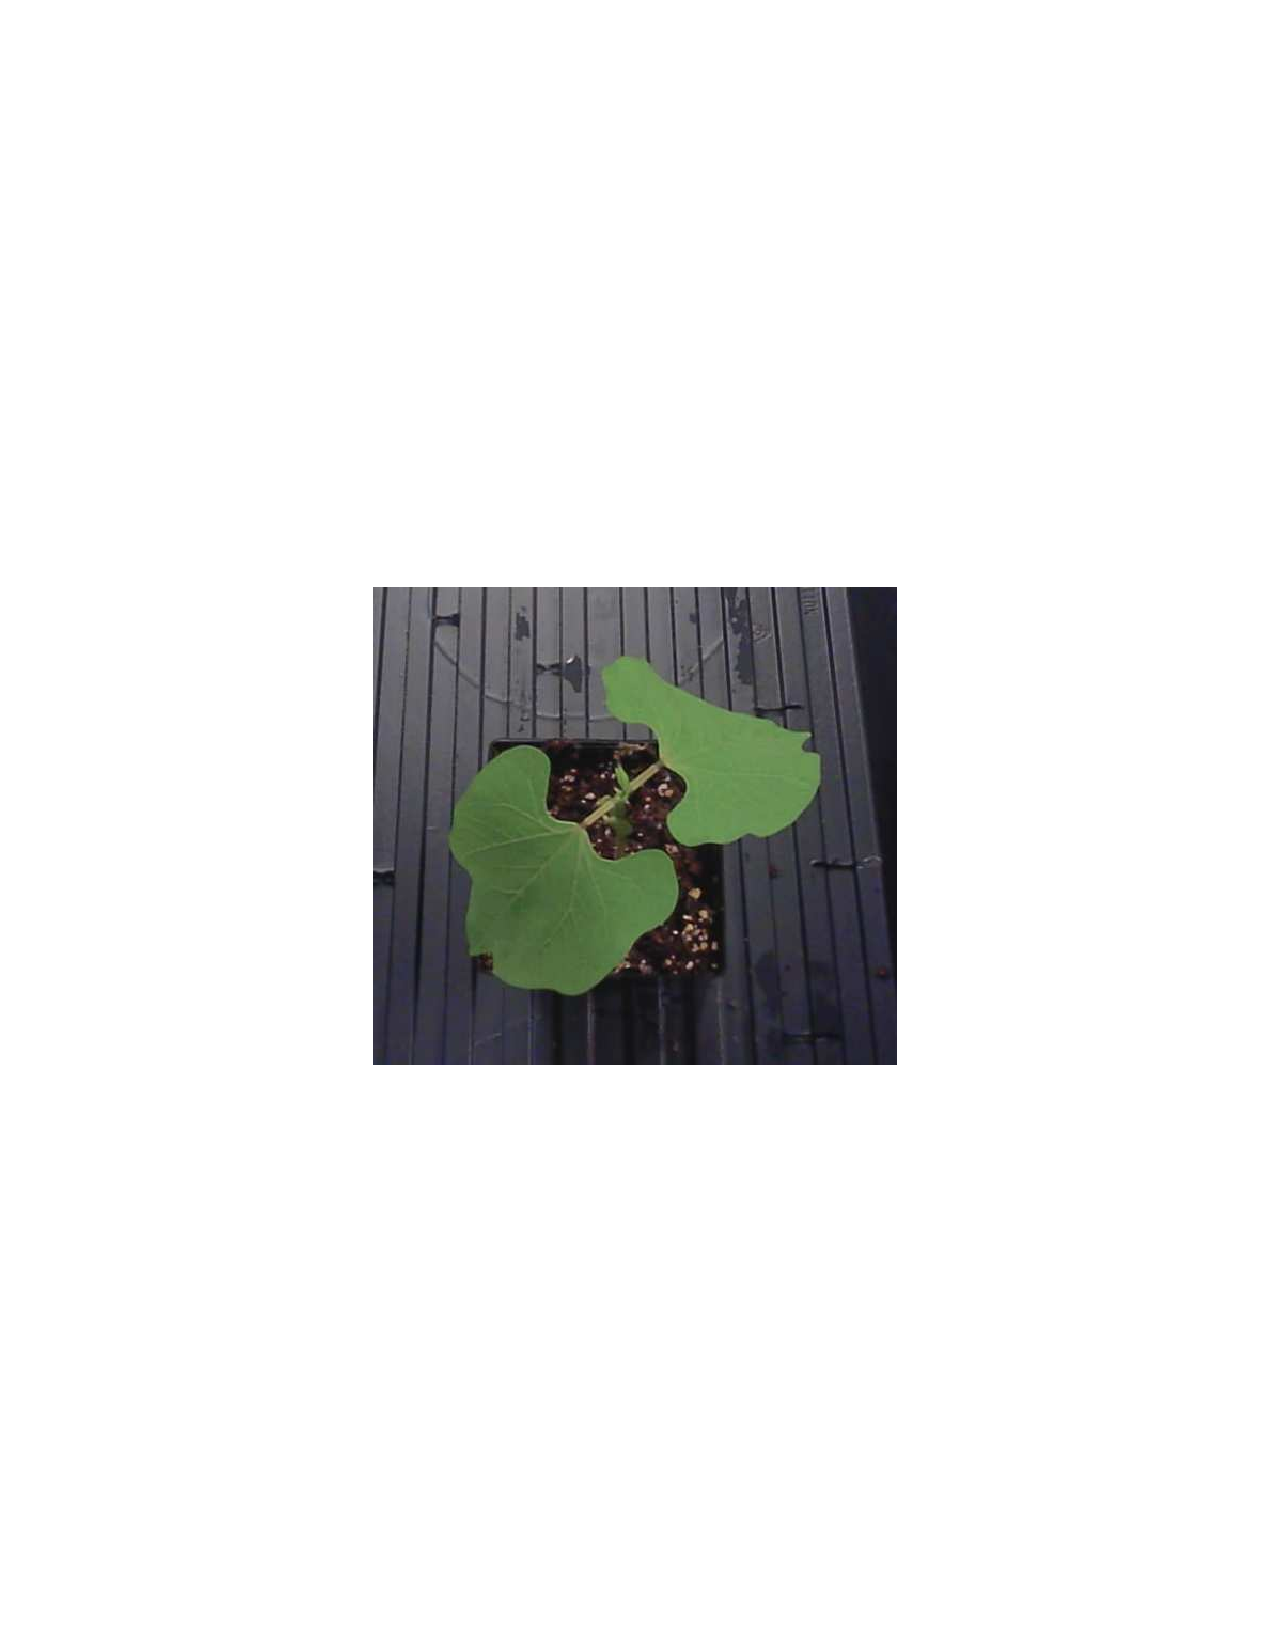
\includegraphics[trim=190 280 190 290,clip,width=0.48\linewidth]{Figures/beanColor} &
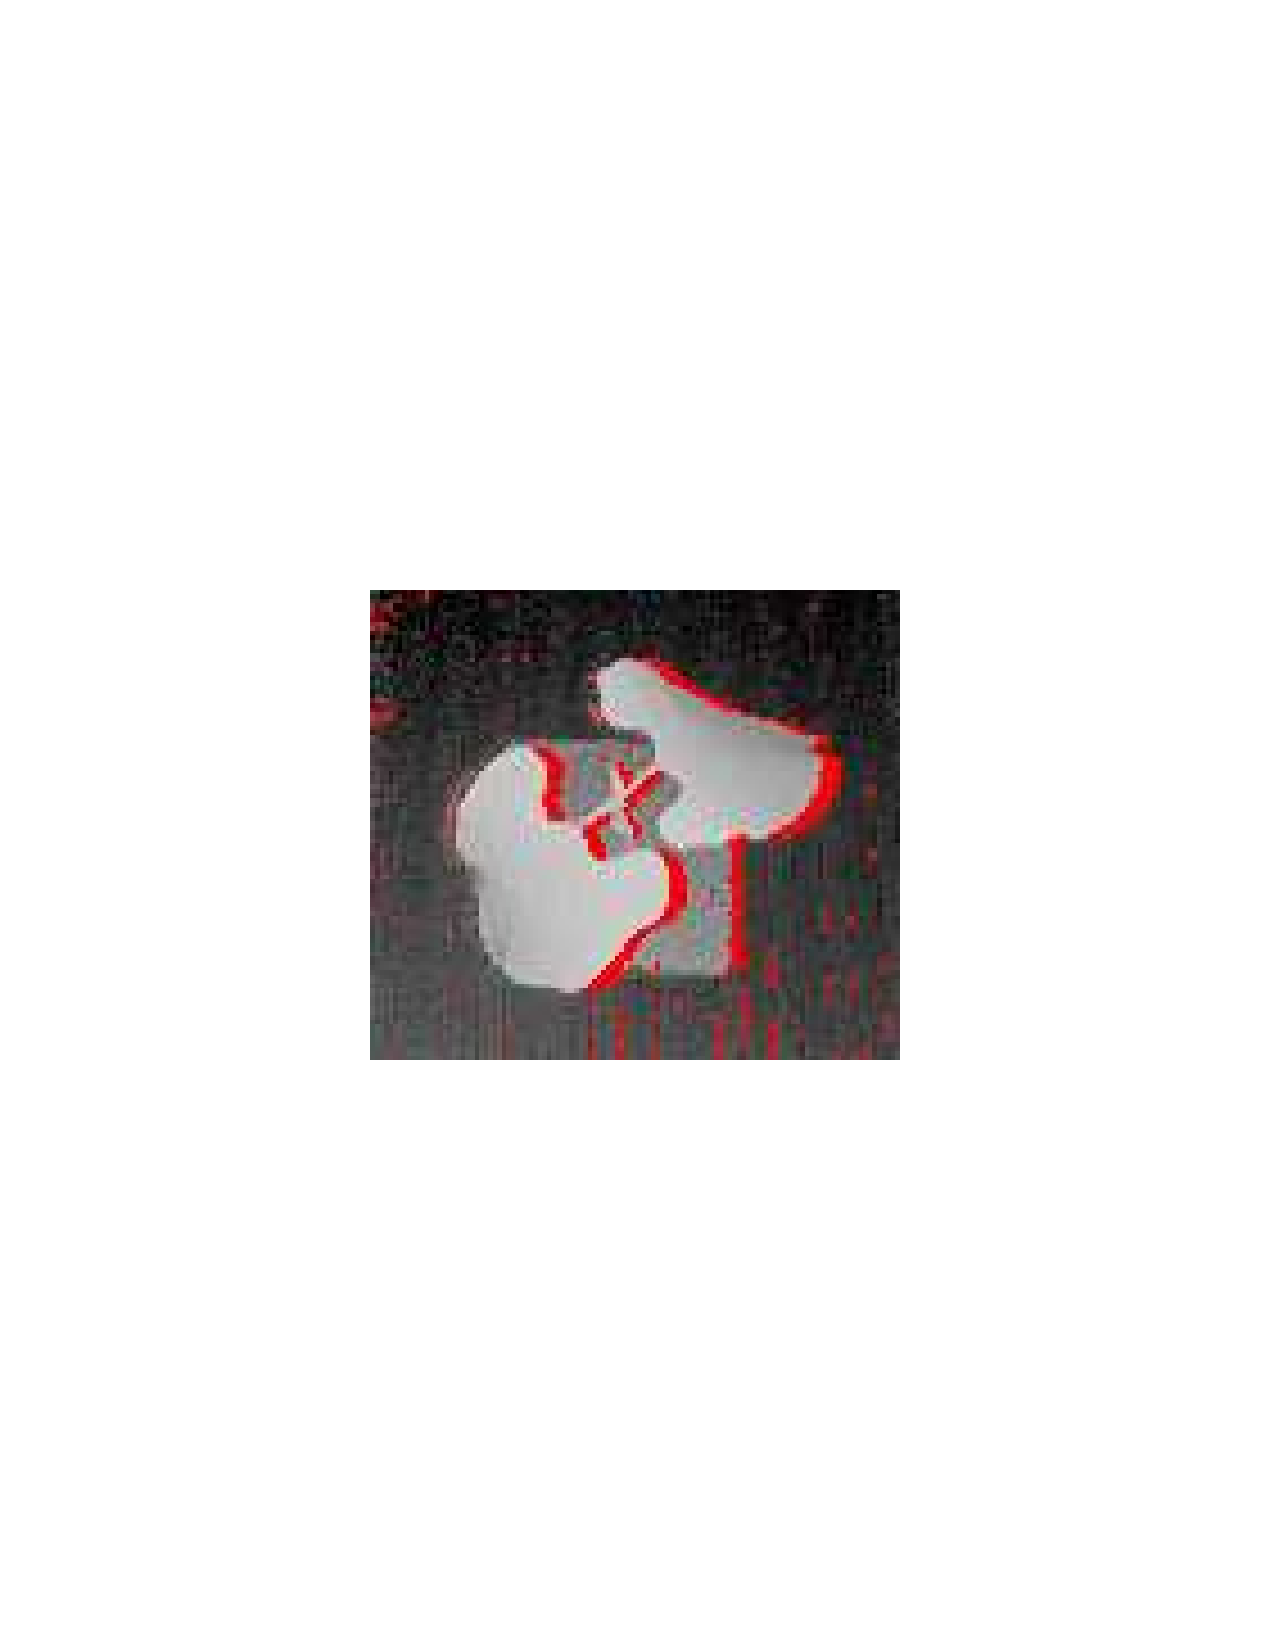
\includegraphics[trim=190 280 190 290,clip,width=0.48\linewidth]{Figures/beanDepth} \\
($a$) & ($b$) \\
%Put bead SLIC and boundary here:
($c$) & ($d$) \\
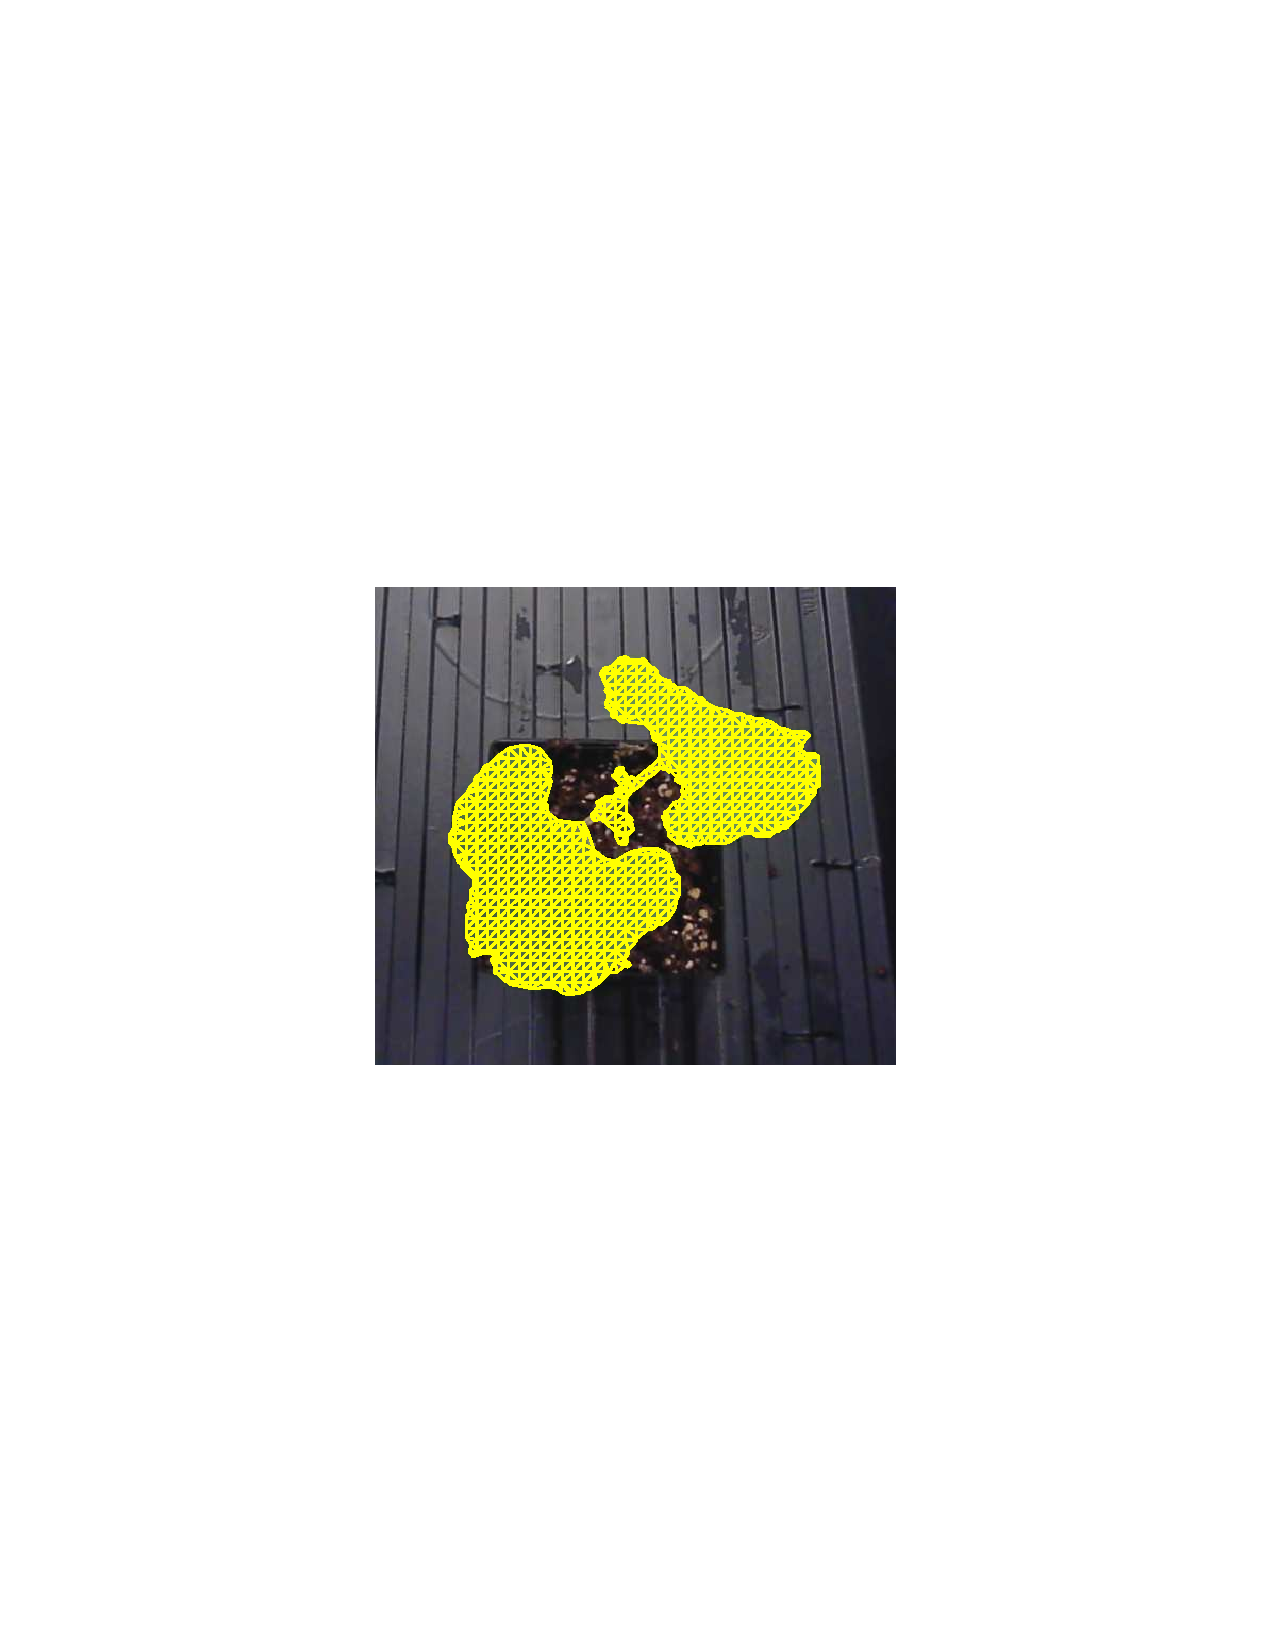
\includegraphics[trim=190 280 190 290,clip,width=0.48\linewidth]{Figures/beanColorMesh} &
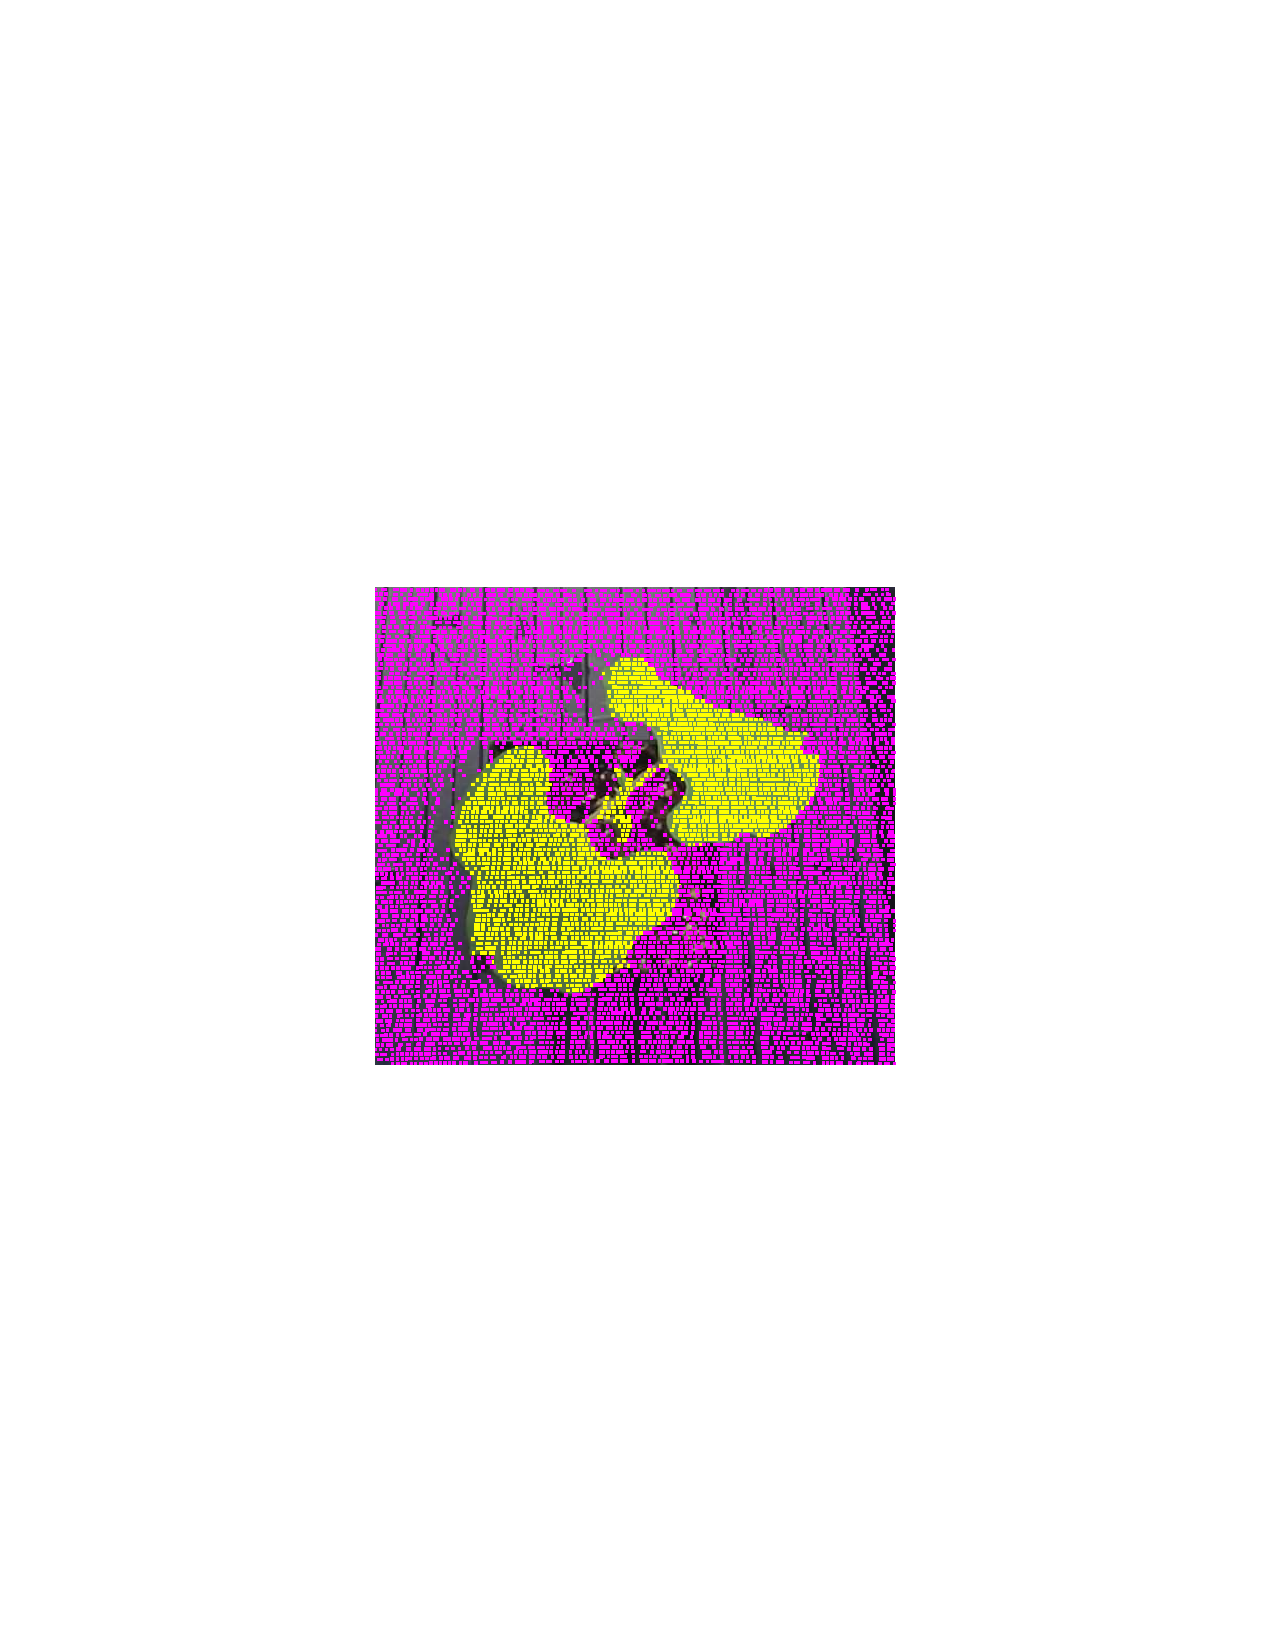
\includegraphics[trim=190 280 190 290,clip,width=0.48\linewidth]{Figures/beanPointsOnLeaves} \\
($e$) & ($f$) \\
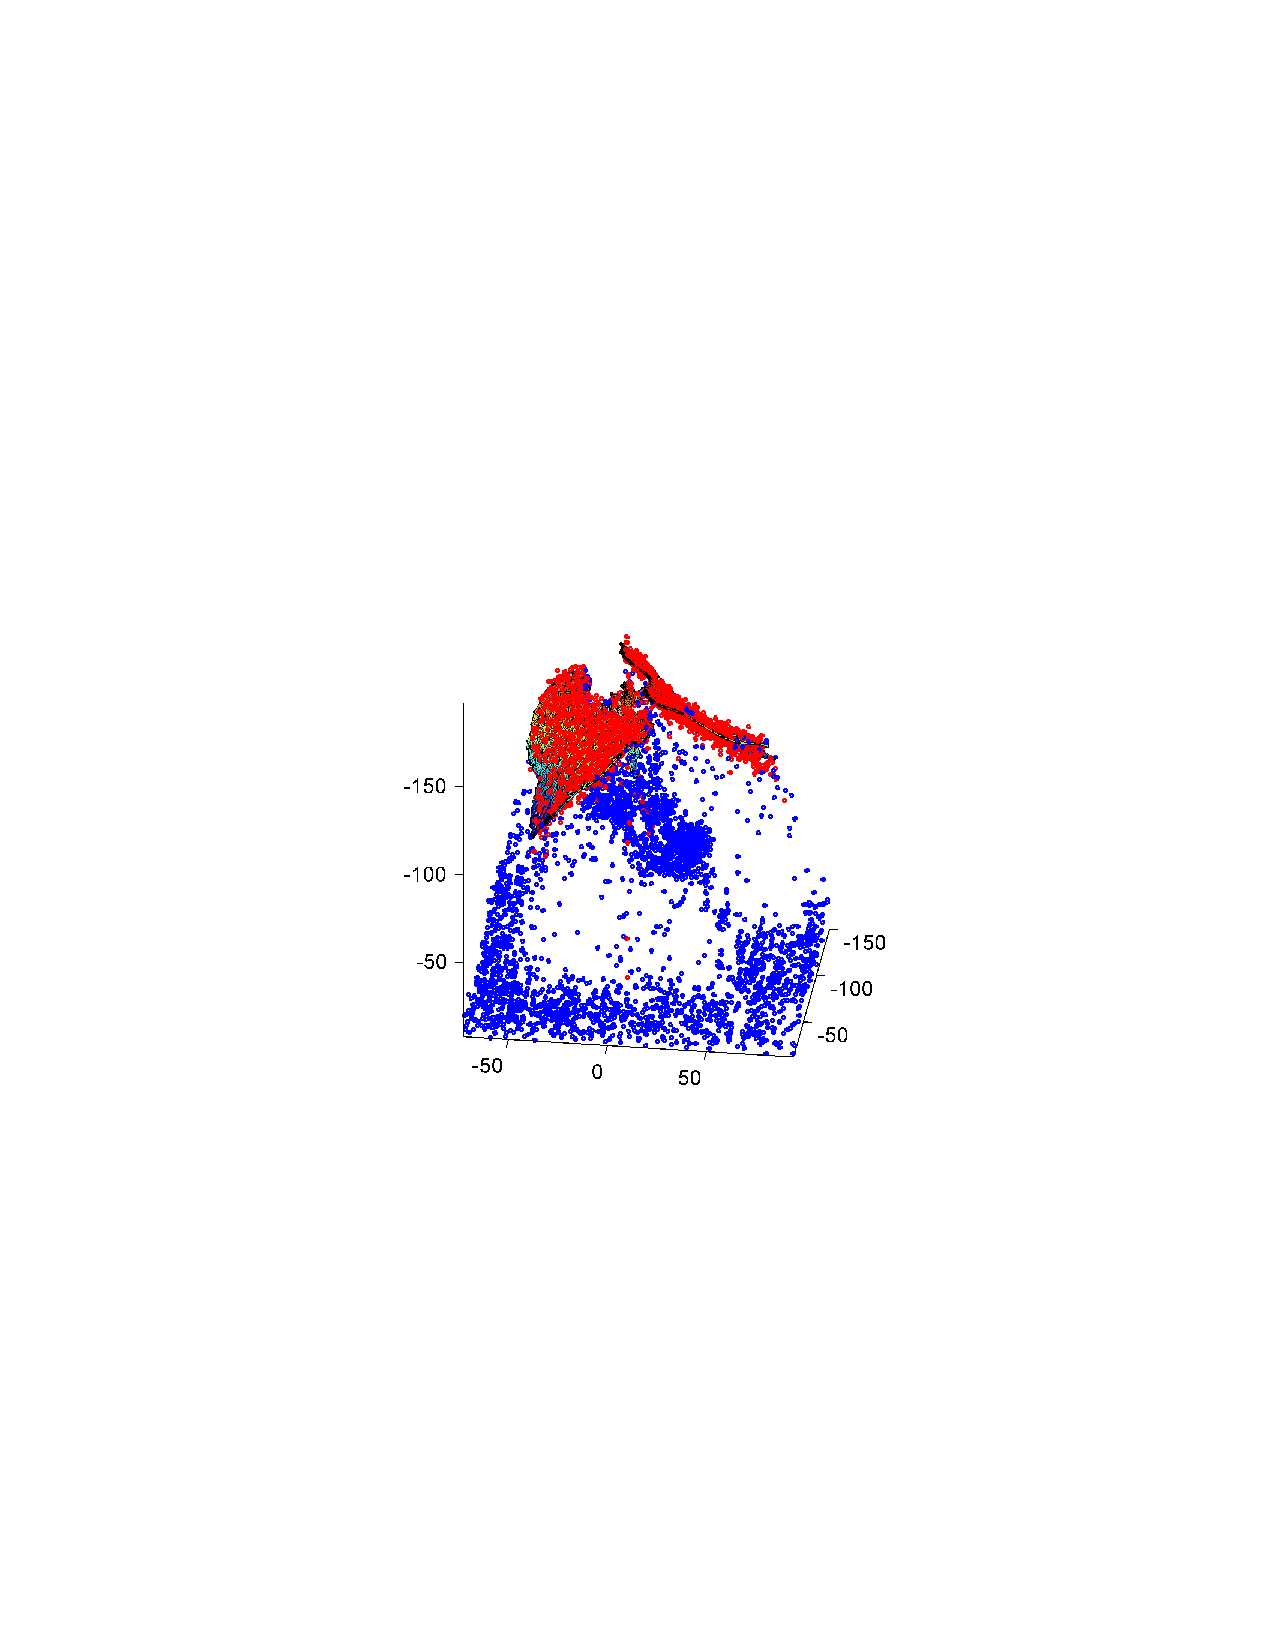
\includegraphics[trim=190 280 190 290,clip,width=0.48\linewidth]{Figures/bean3DMeshPlusPoints} &
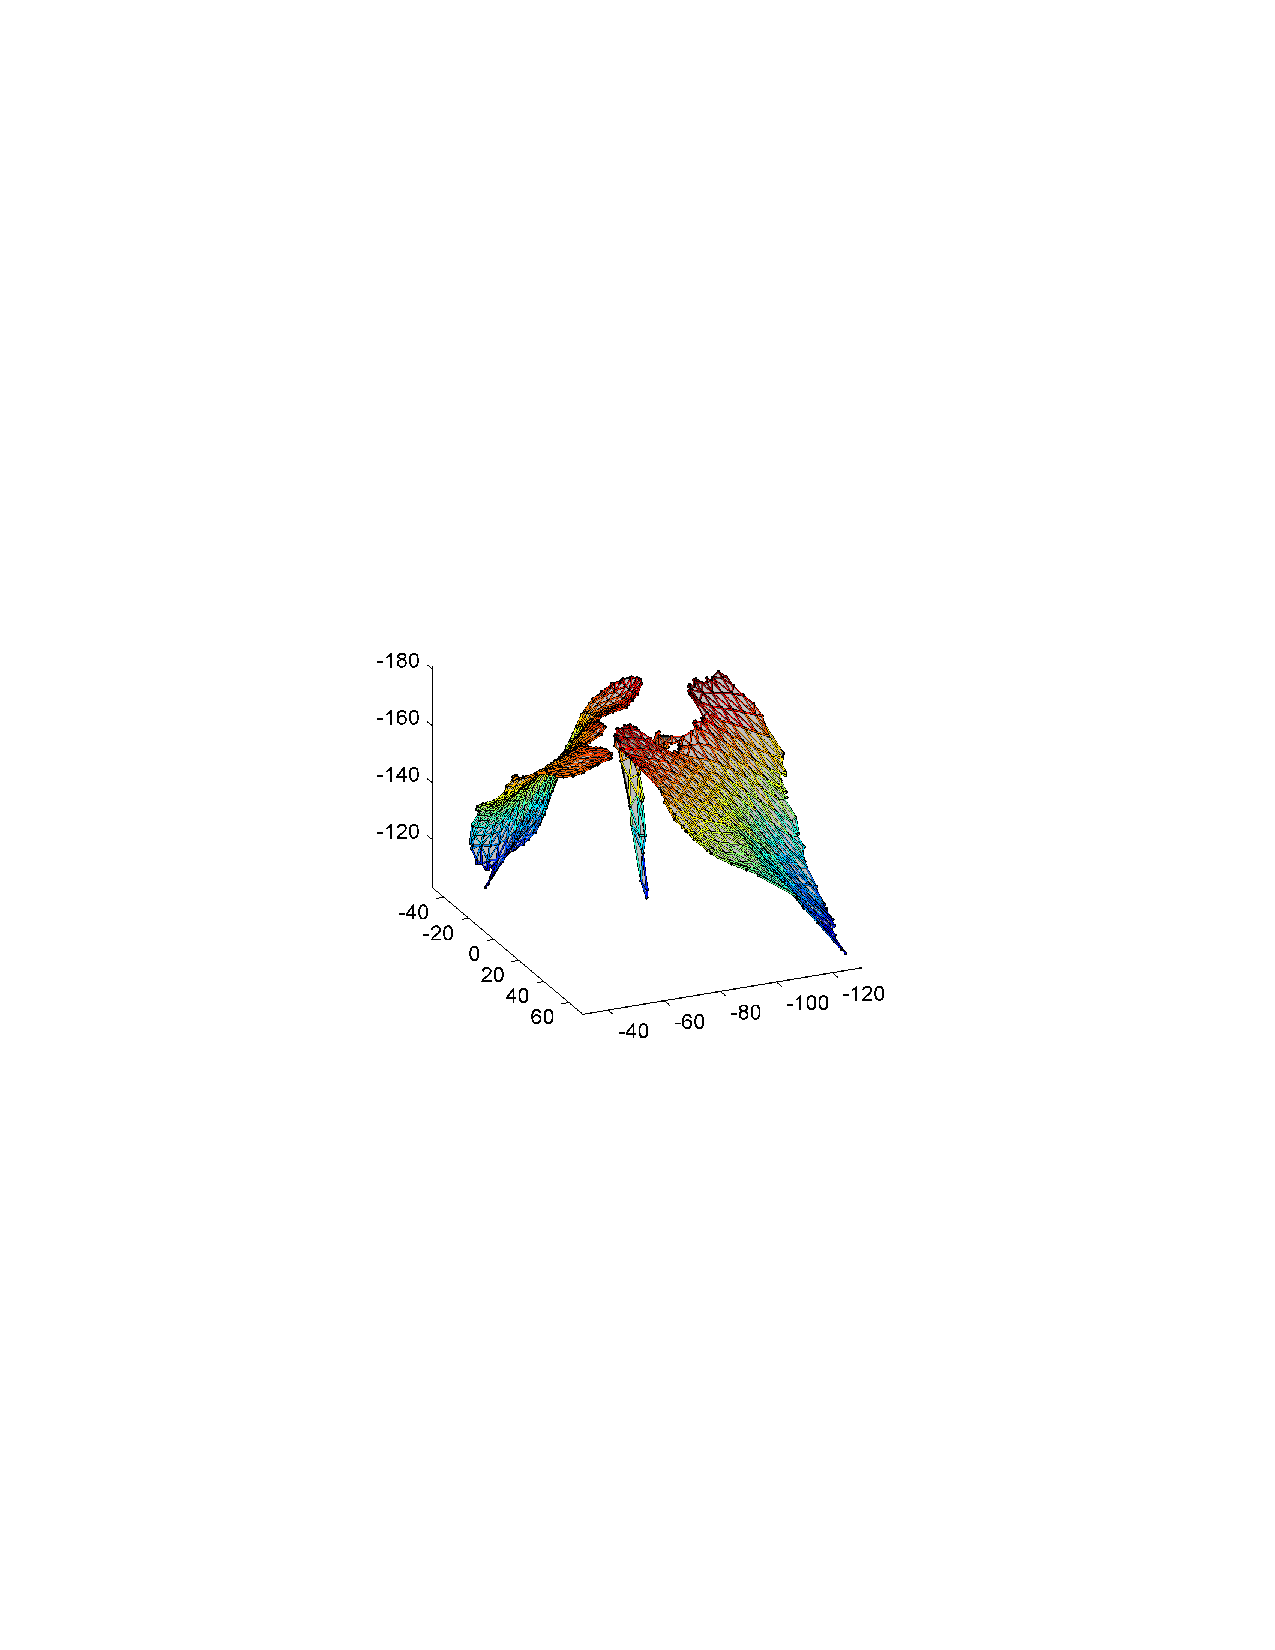
\includegraphics[trim=190 280 190 290,clip,width=0.48\linewidth]{Figures/bean3DMesh} \\
($g$) & ($h$) \\
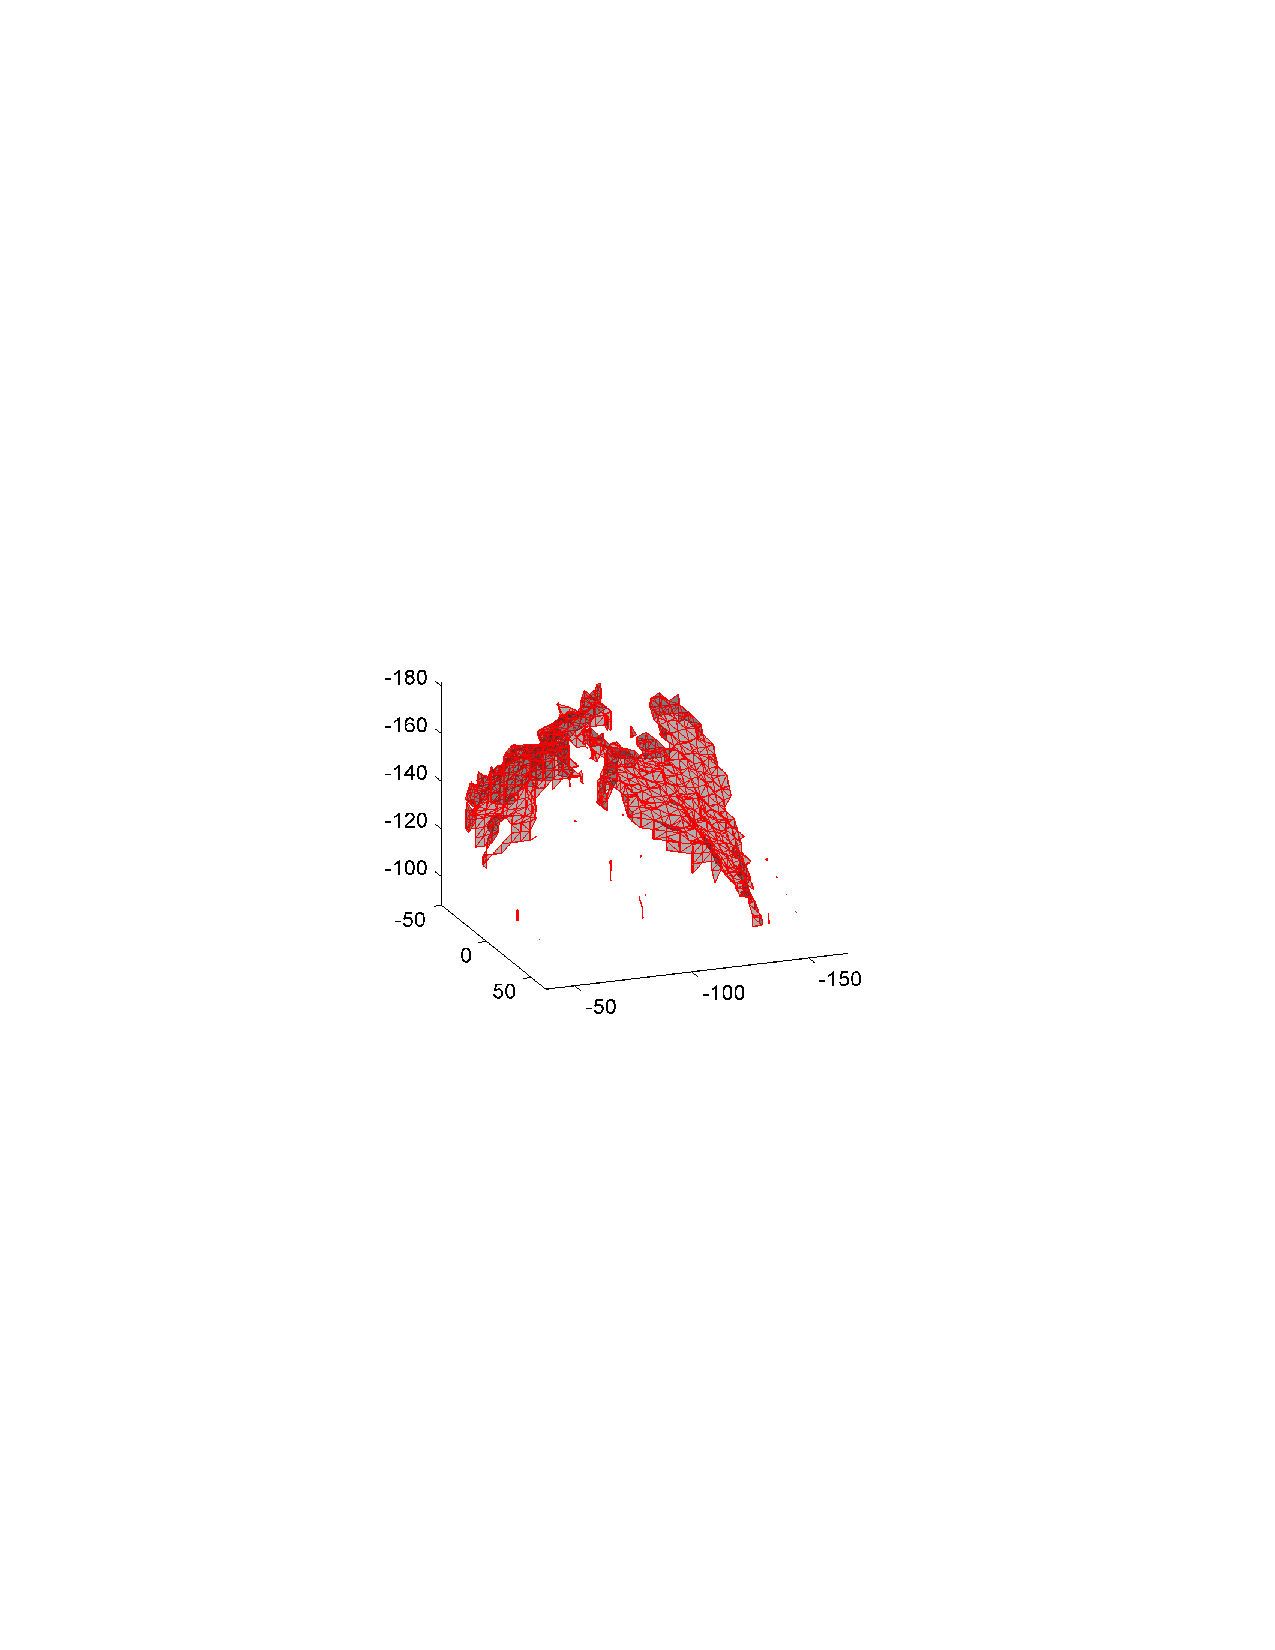
\includegraphics[trim=190 280 190 290,clip,width=0.48\linewidth]{Figures/bean3DIsosurface} & \\
($i$) & ($h$) \\
\end{tabular}
\end{center}
   \caption{The algorithm steps are illustrated.  ($a$) Color image portion on plant.  ($b$) Depth image, where red pixels are those that are masked out using the method in Fig.~\ref{fig:occlusion} as they are not visible in the color image. ($c$) ($d$), ($e$) An mesh is defined in the color image within the leaf boundaries. ($f$) Points that project into the image-mesh, excluding occluded points from ($b$), are shown in yellow over the color image, and the remaining visible points are plotted in magenta.  ($g$) The mesh fit along the vertex rays is shown.  The $3$D points are red for those on the mesh and blue for the remaining.  ($h$) A more detailed view of the mesh. ($i$) A comparison with an isosurface created using marching cubes~\cite{} }
\label{fig:sigmainterframe}
\end{figure}


\begin{figure}
\begin{center}
\begin{tabular}{cc}
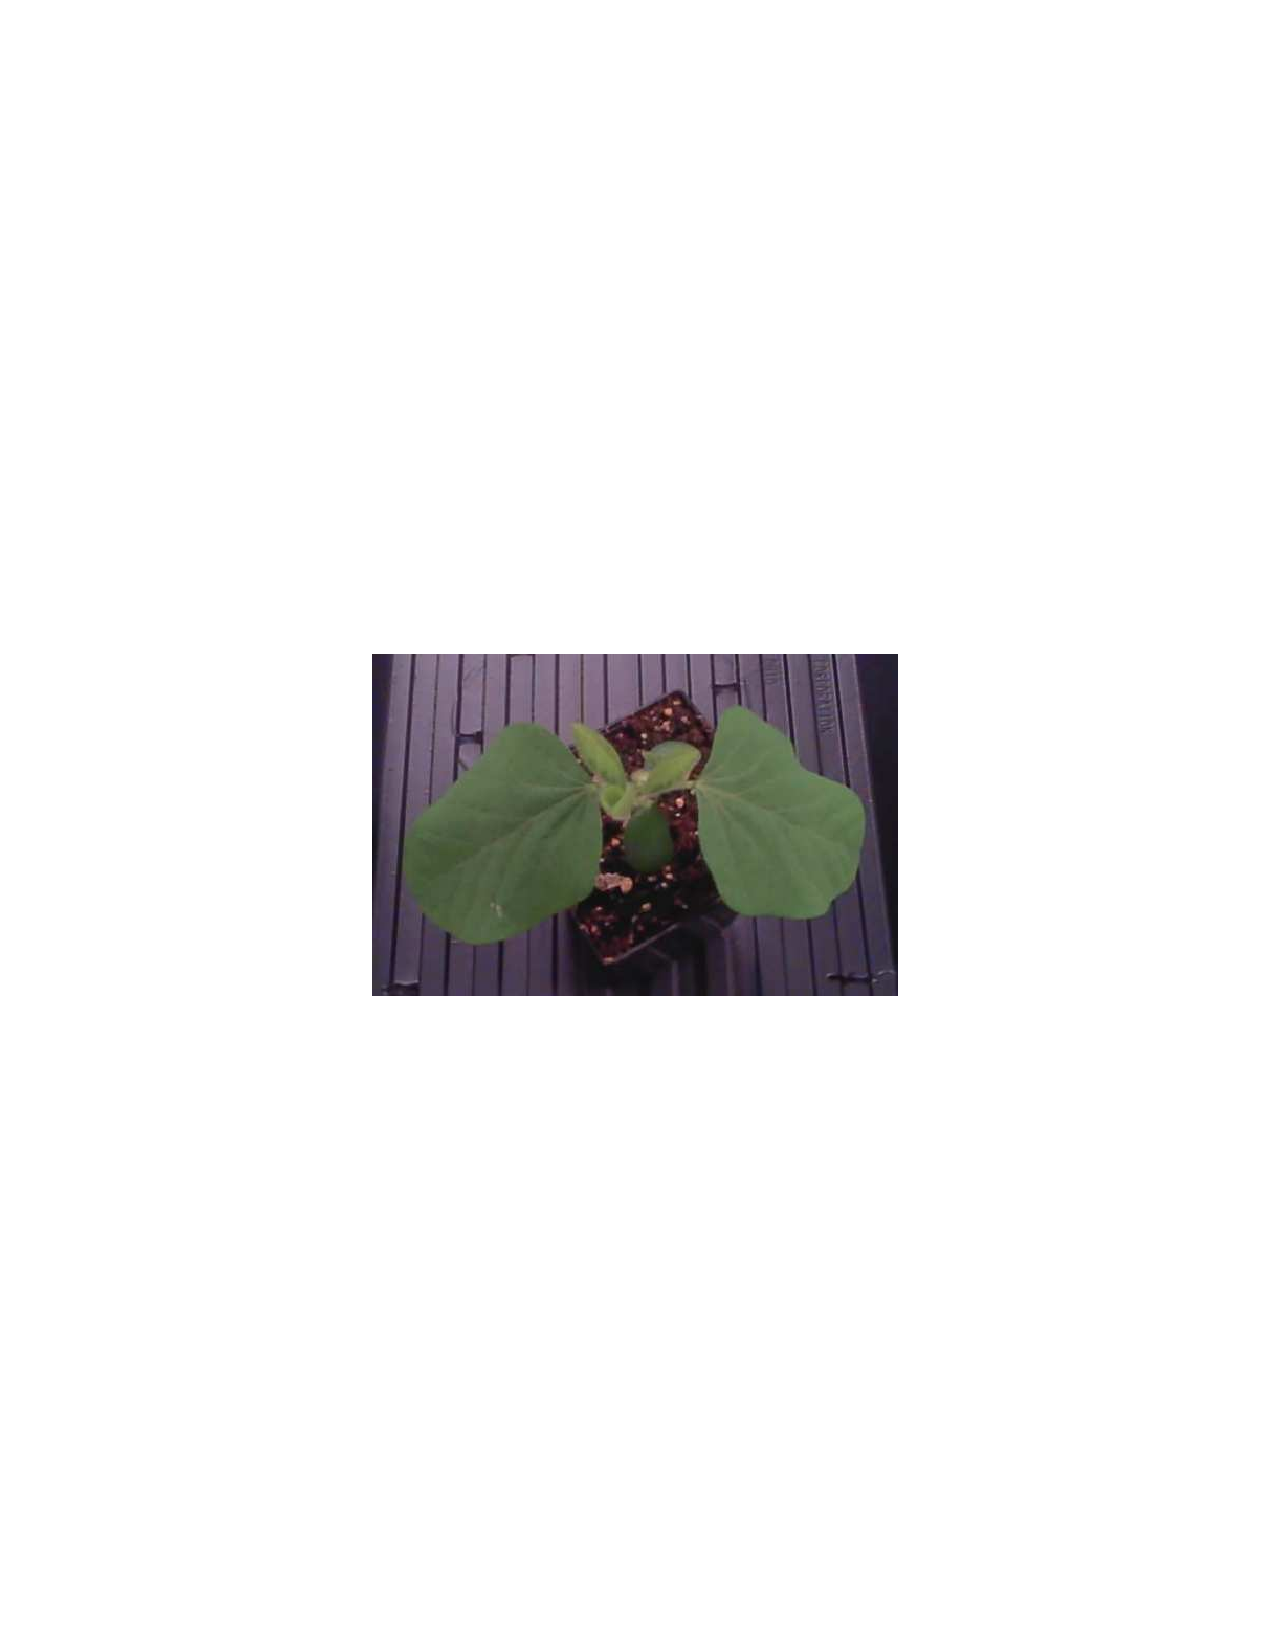
\includegraphics[trim=190 280 190 290,clip,width=0.48\linewidth]{Figures/soybeanColor} &
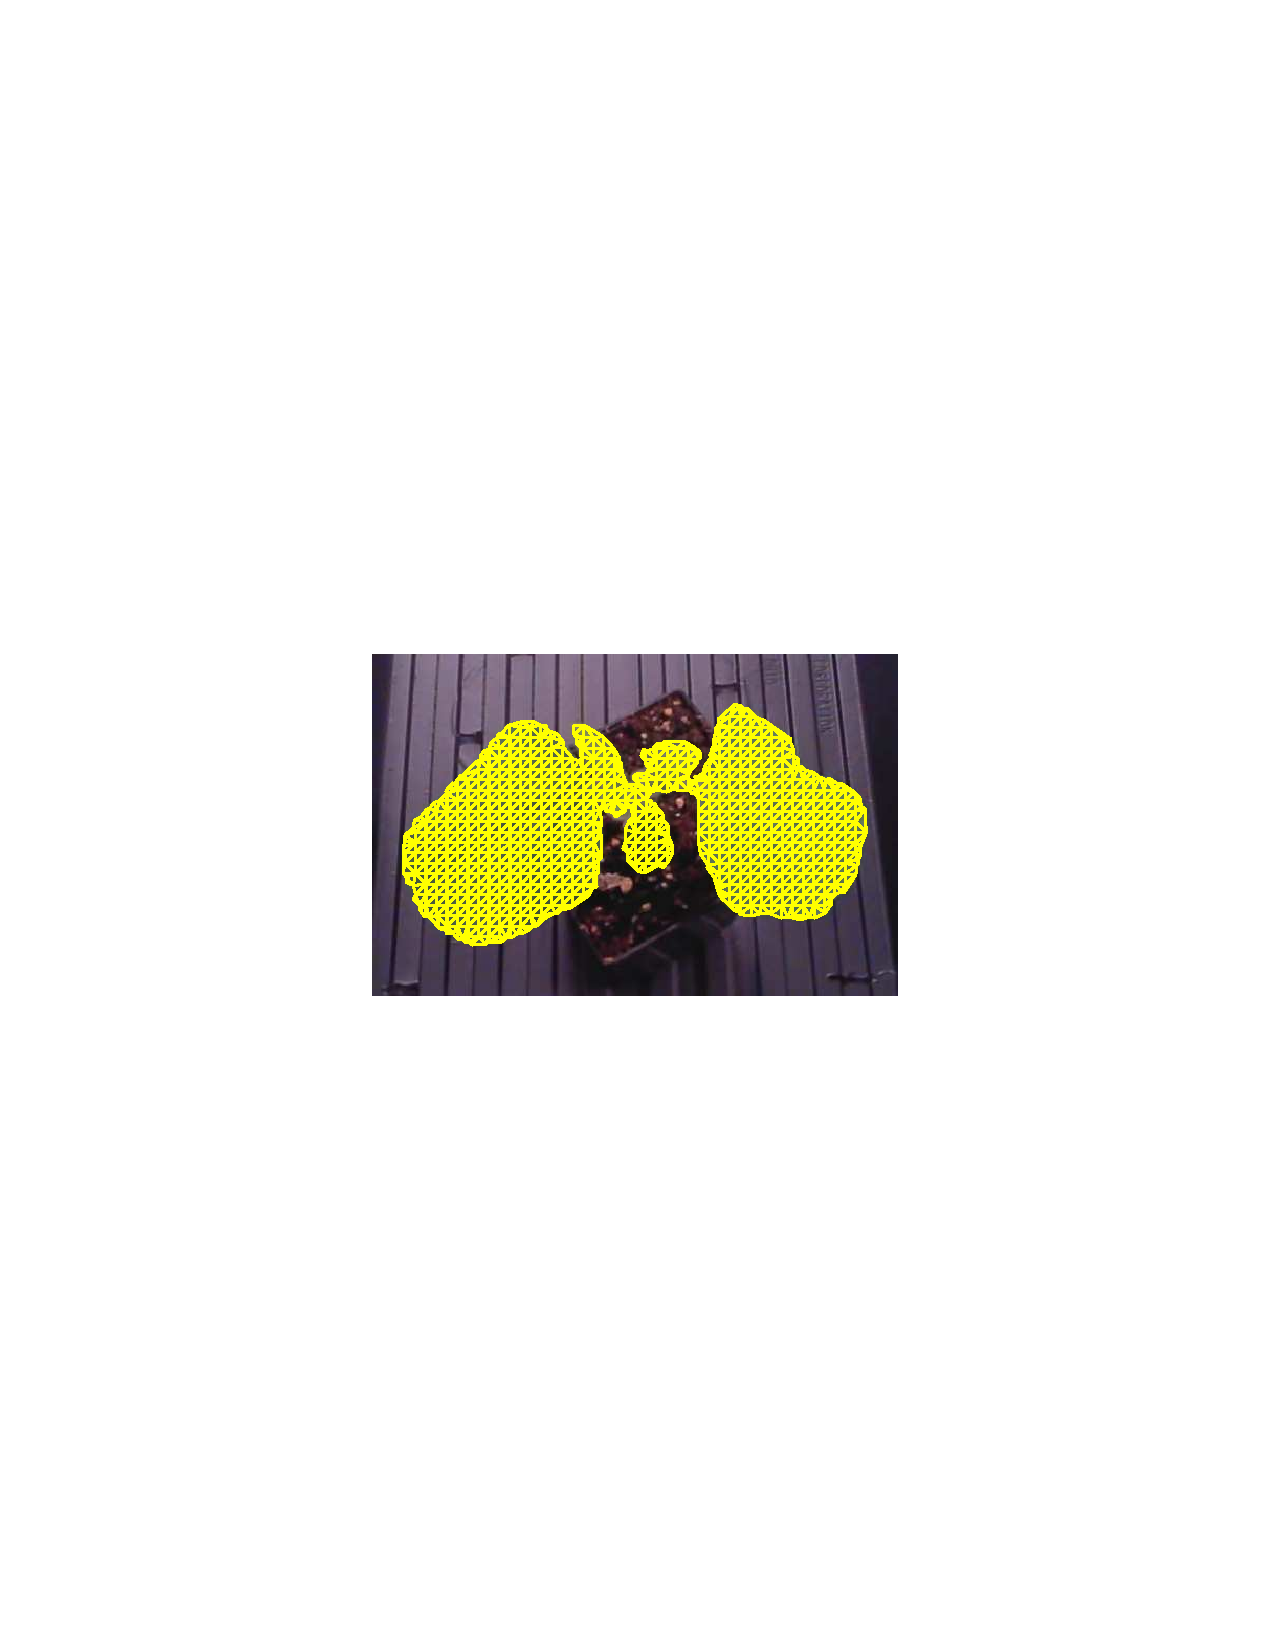
\includegraphics[trim=190 280 190 290,clip,width=0.48\linewidth]{Figures/soybeanColorMesh} \\
($a$) & ($b$) \\
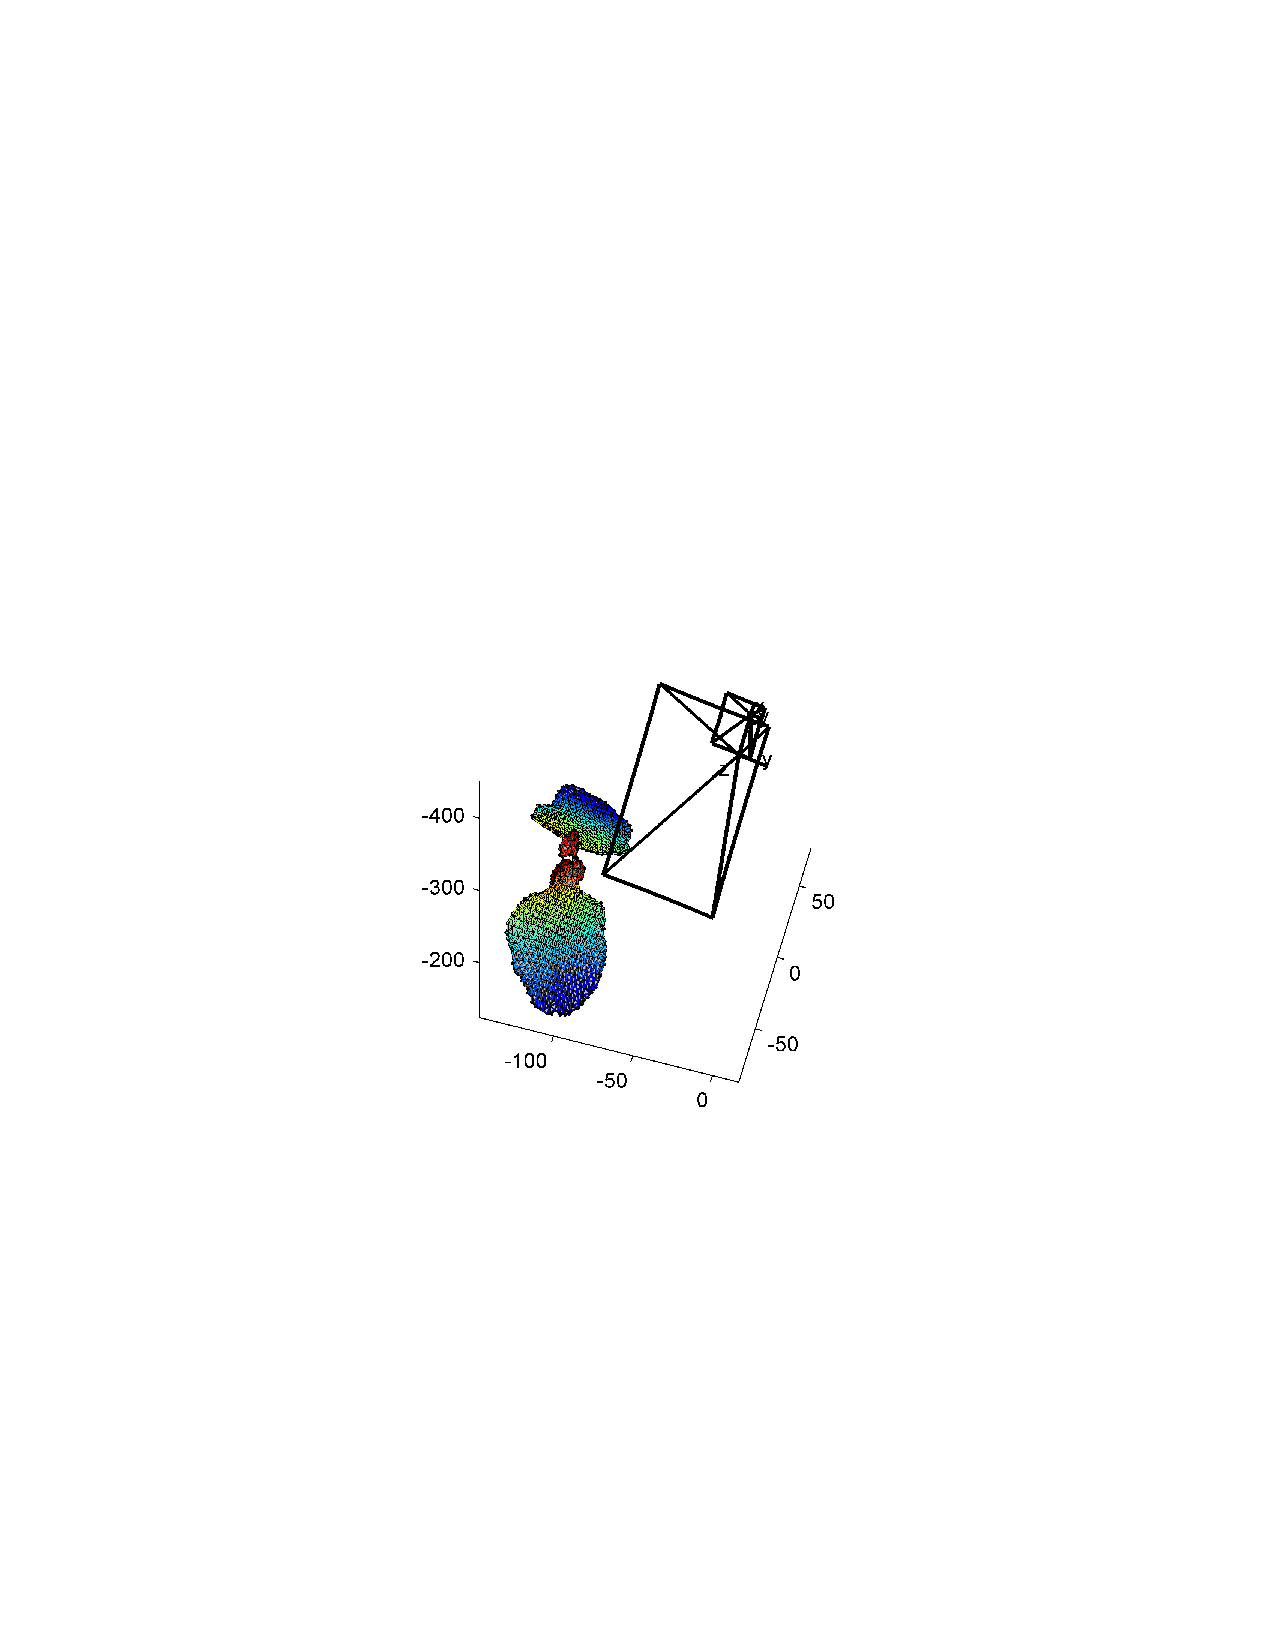
\includegraphics[trim=190 280 190 290,clip,width=0.48\linewidth]{Figures/soybean3DMeshPlusCam} &
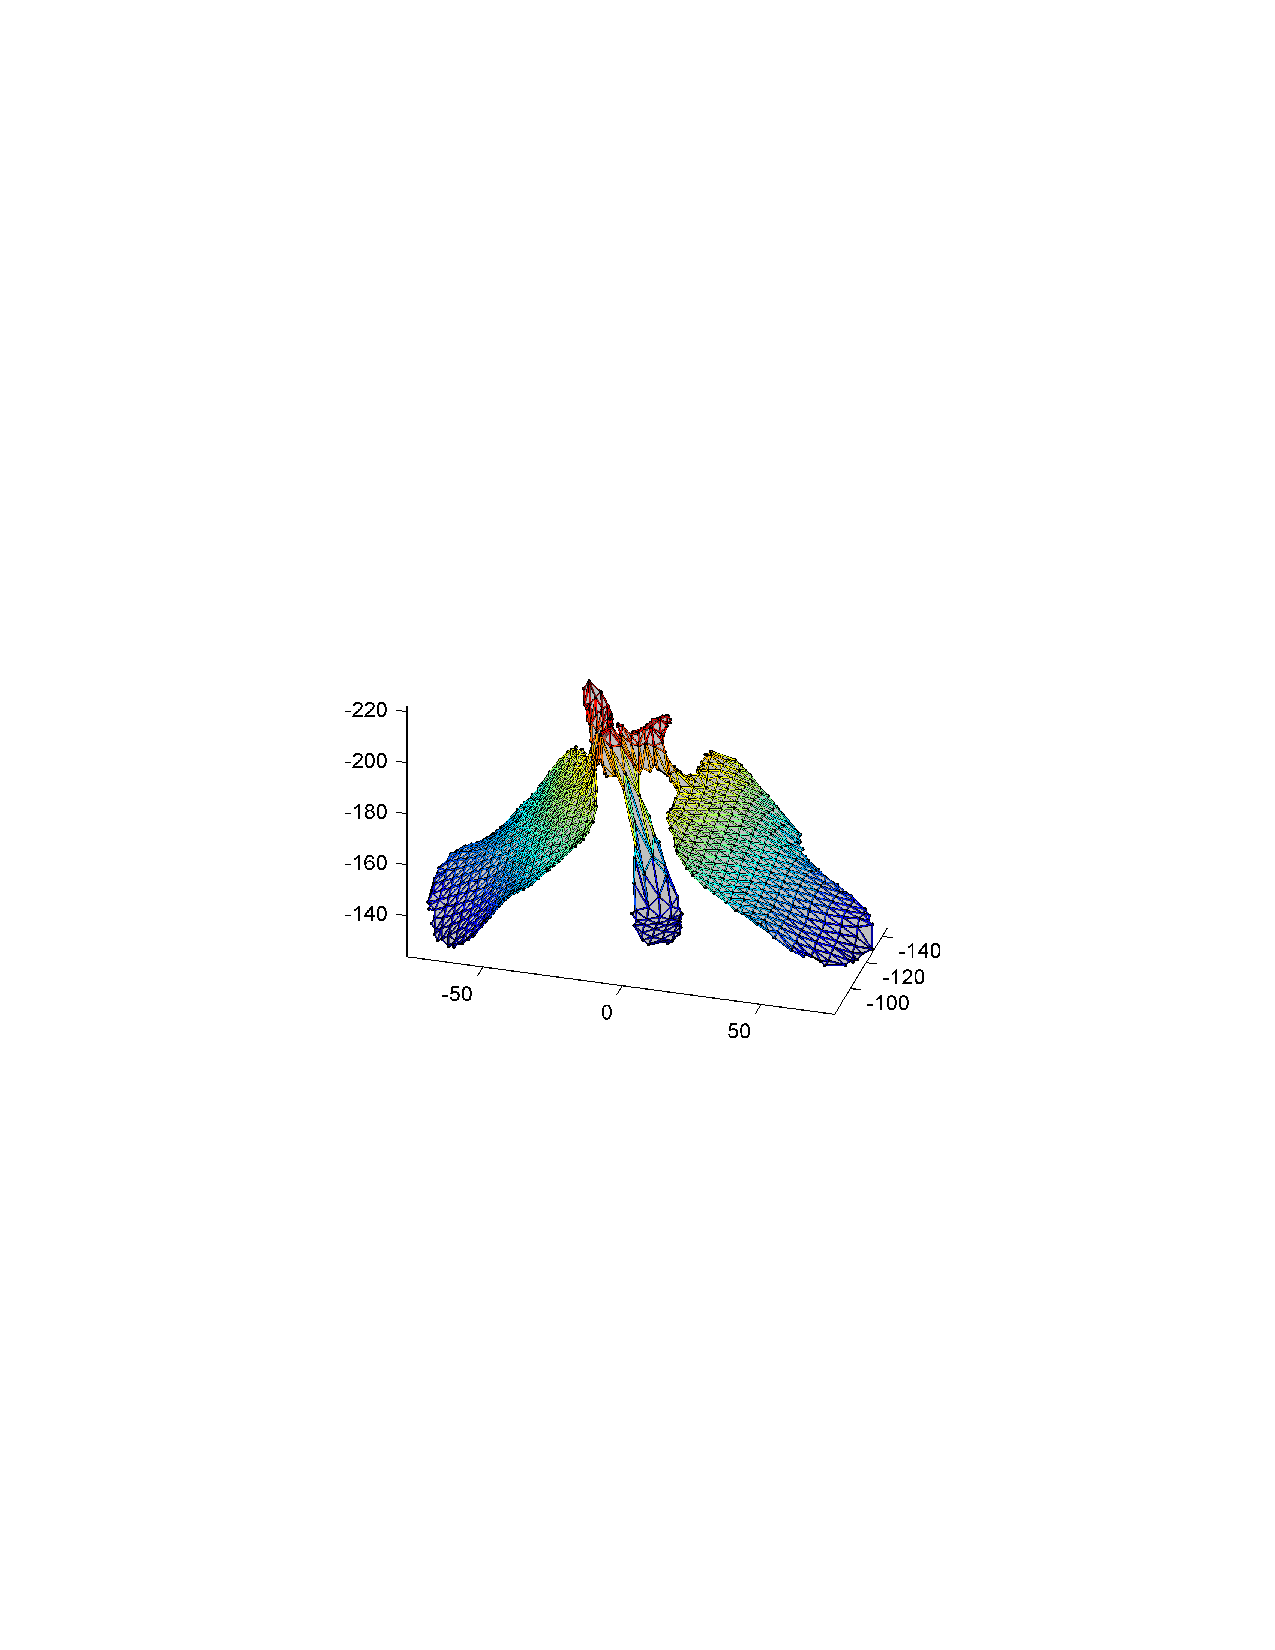
\includegraphics[trim=190 280 190 290,clip,width=0.48\linewidth]{Figures/soybean3DMesh} \\
($c$) & ($d$) \\
\end{tabular}
\end{center}
   \caption{($a$) Color image of a soybean plant.  ($b$) Mesh on the color image. ($c$) $3$D mesh along with camera poses. ($d$) Close-up of $3$D mesh.  }
\label{fig:sigmainterframe}
\end{figure}





\section{Conclusion}
\label{sec:conclusion}

This work presents a new method for estimating high fidelity plant leaf surfaces from RGB-D data.  Our mesh model is flexible enough to capture a wide variety of complex leaf surfaces, and at the same time can filter out significant depth noise from the sensor.  Robustness to noise is achieved by constraining the mesh vertices to fit along the color pixel rays, by minimizing the depth error, and through a curvature-based regularization term.  Results show significant improvement in shape estimation of complex leaves over alternative methods that use voxel models and that use single-leaf geometric primitives. Our future work will involve dealing with overlapping leaves and dense foliage in more cluttered background by using more robust segmentation and leaf detection techniques. We also plan to characterize the mesh region in $3$D world with green pigments and photosynthetic rates by using data from florescent and other high fidelity cameras keeping it adjacent to RGB-D sensors. We anticipate this method will enable automated plant growth observation and further research into improved crop varieties.



%-------------------------------------------------------------------------

{\small
\bibliographystyle{ieee}
\bibliography{sense3d}
}
%-------------------------------------------------------------------------

\end{document}
